\documentclass[twoside,11pt]{article}

% jmlr2e.sty already loads: amssymb, natbib, graphicx, hyperref
\usepackage{jmlr2e}
\usepackage{amsmath}
\usepackage{mathtools}
\usepackage{booktabs}
\usepackage{algorithmic}
\usepackage{algorithm}
\usepackage{lastpage}

% jmlr2e.sty already defines: theorem, proposition, lemma, corollary,
% conjecture, definition, example, remark, proof environments.
% We only add assumption.
\newtheorem{assumption}[theorem]{Assumption}

% Operators
\DeclareMathOperator{\diag}{diag}
\DeclareMathOperator{\tr}{tr}
\DeclareMathOperator{\sign}{sign}
\DeclareMathOperator{\Var}{Var}
\DeclareMathOperator{\Cov}{Cov}
\DeclareMathOperator{\HSIC}{HSIC}
\DeclareMathOperator{\argmin}{arg\,min}

% Shortcuts
\newcommand{\R}{\mathbb{R}}
\newcommand{\C}{\mathbb{C}}
\newcommand{\N}{\mathbb{N}}
\newcommand{\bx}{\mathbf{x}}
\newcommand{\be}{\mathbf{e}}
\newcommand{\bone}{\mathbf{1}}
\newcommand{\SCC}{\mathrm{SCC}}
\newcommand{\SCD}{\mathrm{SCD}}
\newcommand{\CCI}{\mathrm{CCI}}
\newcommand{\DPI}{\mathrm{DPI}}
\newcommand{\ECD}{\mathrm{ECD}}

% JMLR heading (placeholders for submission)
\jmlrheading{}{2026}{1-\pageref{LastPage}}{5/14}{}{}{Tatsuki Onishi}

\ShortHeadings{Spectral Causality via Magnetic Laplacians}{Onishi}
\firstpageno{1}

\begin{document}

\title{Spectral Causality: Causal Direction Estimation via \\
Magnetic Laplacians and Hodge Decomposition}

\author{\name Tatsuki Onishi \email bougtoir@gmail.com \\
       \addr Data Science and AI Innovation Research Promotion Center \\
       Shiga University, Japan}

\editor{TBD}

\maketitle

\begin{abstract}%
I introduce \emph{spectral causality}, a framework for causal direction
estimation via the \emph{magnetic Laplacian}, an Hermitian matrix whose
complex-valued eigenvectors encode edge directionality as phase.  I define
a \emph{Directional Predictability Index} (DPI) that resolves the
circularity of earlier utility-based formulations: under additive noise
model assumptions, DPI consistently estimates causal direction without
domain knowledge.  Connecting the framework to \emph{Hodge decomposition},
I prove that gradient--curl--harmonic separation of edge flows yields a
causal potential recovering topological order under directed acyclic graph
(DAG) structure, and establish \emph{scale invariance} of the gradient
energy ratio $r_{\mathrm{gradient}}$, showing that causal structure
emergence depends on knowledge \emph{quality} rather than quantity.
Experiments on synthetic random DAGs ($n{=}5$--$20$, $N{=}200$--$1000$),
the Sachs protein signaling network ($n{=}11$, 17~ground-truth edges),
and the UCI Heart Disease dataset ($N{=}297$, 5~variables) demonstrate
competitive recovery against DirectLiNGAM, the PC algorithm, GES, and
NOTEARS.  On Sachs data with partial knowledge, spectral causality achieves
a true positive rate (TPR) of~$0.56$ and a false discovery rate (FDR)
of~$0.27$, while providing unique DAG-adequacy diagnostics and detecting
feedback loops invisible to DAG-based methods.
\end{abstract}

\begin{keywords}
Causal discovery, Magnetic Laplacian, Hodge decomposition, Spectral graph theory, Directed graphs
\end{keywords}

%% ============================================================
\section{Introduction}
\label{sec:intro}

Causal inference---determining whether $X$ causes $Y$---is a central problem
in science and medicine.  The dominant approaches include structural equation
models (SEMs) with the $do$-calculus \citep{Pearl2009}, potential outcomes
\citep{Rubin1974}, the linear non-Gaussian acyclic model (LiNGAM)
\citep{Shimizu2006}, and Granger causality for time series
\citep{Granger1969}.

This paper proposes a fundamentally different principle: \emph{reading causal
directions from the spectral structure (eigenvalues and eigenvectors) of a
graph Laplacian}.  I call this approach \textbf{spectral causality}.

\paragraph{Basic idea.}
Given $n$ variables $\{X_1,\dots,X_n\}$ with putative causal relations
represented as a weighted directed graph $G=(V,E,w)$, the \emph{magnetic
Laplacian} $\mathcal{L}^{(q)}$ is an Hermitian matrix whose eigenvectors are
complex-valued.  The \emph{phase angles} of these eigenvectors encode edge
directionality, enabling estimation of causal direction from spectral
structure alone.

\paragraph{Key distinction from DAG-based methods.}
LiNGAM and related methods assume a directed acyclic graph (DAG).  In
biomedical systems, feedback loops are ubiquitous (e.g., inflammation
$\to$ organ damage $\to$ inflammation).  Spectral causality accommodates
\emph{directed cyclic graphs} (DCGs) via the Hodge decomposition, which
separates gradient (DAG-like) and curl (feedback) components of causal flow.

\paragraph{Contributions.}
The main contributions of this paper are:

\begin{enumerate}
\item \textbf{Directional Predictability Index (DPI).}  A data-driven
  asymmetric statistic that enables causal direction estimation at $\alpha=0$
  (no domain knowledge), resolving the circularity in earlier utility-based
  formulations (Section~\ref{sec:formulation}).

\item \textbf{DAG-free causal inference.}  Via Hodge decomposition, I
  separate DAG-compatible flow (gradient) from feedback (curl), providing
  the gradient energy ratio $r_{\mathrm{gradient}}$ as a quantitative
  measure of DAG adequacy (Section~\ref{sec:hodge}).

\item \textbf{Scale invariance theorem.}  I prove that
  $r_{\mathrm{gradient}}$ depends only on the \emph{structure} (sign
  pattern) of the asymmetric component of the utility matrix, not on its
  magnitude---establishing that knowledge \emph{quality}, not quantity,
  governs causal structure emergence (Section~\ref{sec:transition}).

\item \textbf{Ensemble Causal Direction (ECD).}  A pipeline integrating
  LiNGAM's local identifiability with spectral causality's global structural
  analysis, achieving broad coverage of Hill's nine epidemiological criteria
  (Section~\ref{sec:ecd}).

\item \textbf{Partial identifiability of DPI.}  Under the additive noise
  model (ANM), the ANM component of DPI consistently identifies causal direction
  as $n\to\infty$, providing a non-circular theoretical foundation
  (Section~\ref{sec:identifiability}).

\item \textbf{Multi-dataset validation.}  Experiments on synthetic random
  DAGs ($n=5$--$20$), the Sachs protein signaling network
  (\citealp{Sachs2005}; $n=11$, 17 ground-truth edges), and the UCI Heart
  Disease dataset ($N=297$, 5 variables) demonstrate competitive
  structural recovery against DirectLiNGAM, the PC algorithm, GES, and
  NOTEARS (Section~\ref{sec:experiments}).
\end{enumerate}

Figure~\ref{fig:three-approaches} provides a conceptual overview of the
three complementary approaches unified in this work.

\begin{figure}[t]
\centering
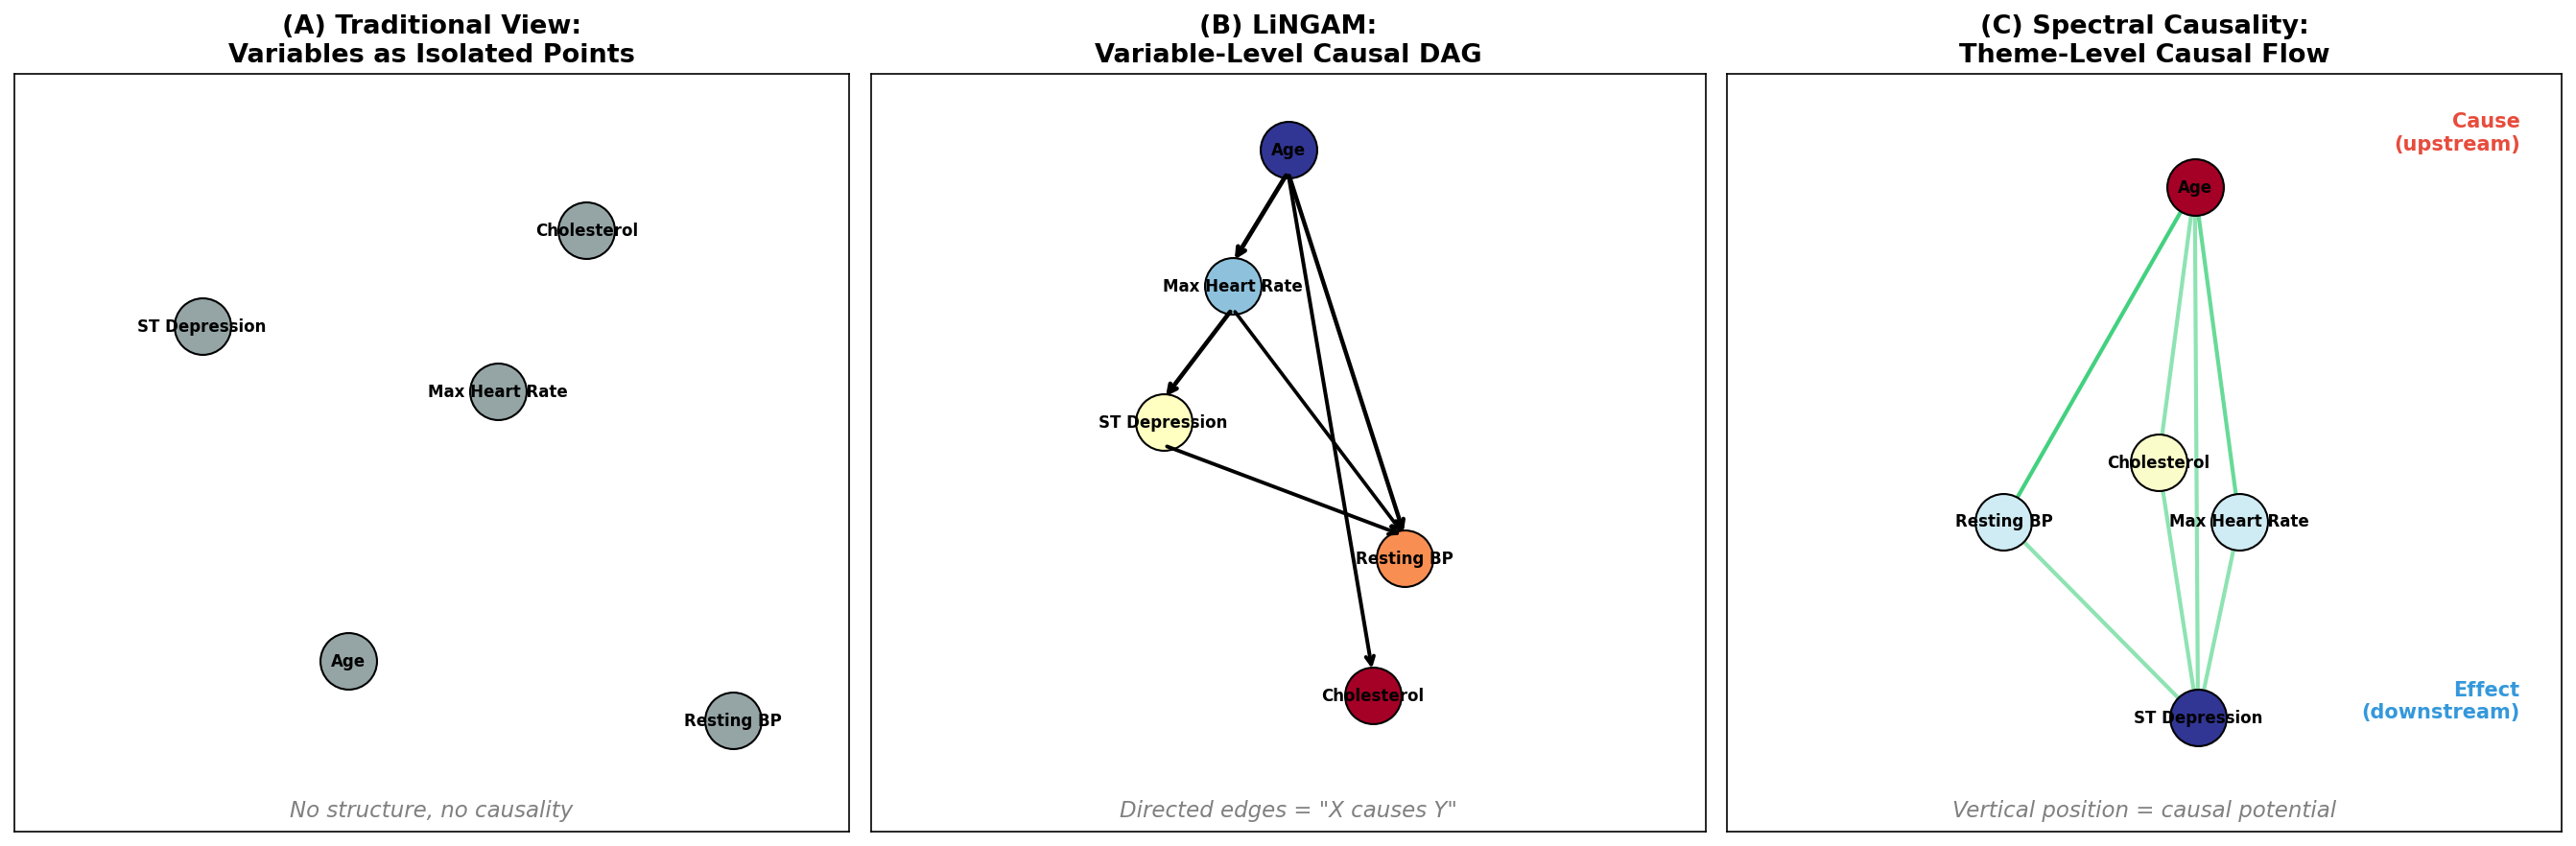
\includegraphics[width=0.85\textwidth]{figures/fig1_three_approaches.png}
\caption{Three complementary approaches to causal inference: (1)~structural
  equation models and DAG-based methods (e.g., LiNGAM), (2)~spectral
  graph methods via the magnetic Laplacian, and (3)~Hodge-theoretic flow
  decomposition.  Spectral causality unifies (2) and (3).}
\label{fig:three-approaches}
\end{figure}

\paragraph{Paper outline.}
Section~\ref{sec:prelim} reviews graph Laplacians.
Section~\ref{sec:magnetic} introduces the magnetic Laplacian.
Section~\ref{sec:formulation} formulates spectral causality and DPI.
Section~\ref{sec:hodge} develops the Hodge decomposition connection.
Section~\ref{sec:related} surveys related work.
Section~\ref{sec:experiments} presents experiments.
Section~\ref{sec:transition} analyzes the DAG phase transition.
Section~\ref{sec:ecd} describes the ECD pipeline.
Section~\ref{sec:identifiability} addresses identifiability.
Section~\ref{sec:discussion} discusses limitations and future work.

%% ============================================================
\section{Preliminaries: Graph Laplacians}
\label{sec:prelim}

\begin{definition}[Graph Laplacian]
\label{def:laplacian}
Let $G=(V,E,w)$ be a weighted undirected graph with $|V|=n$ and weight
function $w:E\to\R_{>0}$.  The \emph{weighted adjacency matrix}
$W\in\R^{n\times n}$, the \emph{degree matrix}
$D=\diag(d_1,\dots,d_n)$ with $d_i=\sum_j W_{ij}$, and the
\emph{graph Laplacians} are:
\[
  L = D - W \quad\text{(unnormalized)}, \qquad
  \mathcal{L} = I - D^{-1/2}WD^{-1/2} \quad\text{(normalized)}.
\]
\end{definition}

\begin{proposition}[Basic properties]
\label{prop:laplacian-basic}
The following hold:
\begin{enumerate}
\item[\emph{(i)}] $L$ is symmetric positive semidefinite with eigenvalues
  $0=\lambda_1\le\lambda_2\le\dots\le\lambda_n$.
\item[\emph{(ii)}] The eigenvector for $\lambda_1=0$ is
  $\bone=(1,\dots,1)^\top$.
\item[\emph{(iii)}] $\lambda_2>0$ if and only if $G$ is connected
  (algebraic connectivity / Fiedler value).
\item[\emph{(iv)}] For any $f\in\R^n$,
  $f^\top Lf = \sum_{(i,j)\in E}w_{ij}(f_i-f_j)^2 \ge 0$.
\end{enumerate}
\end{proposition}

\begin{proof}
Property~(iv) follows by expanding the quadratic form of $L=D-W$.
Property~(i) is immediate from~(iv).  Property~(ii) holds since
$L\bone=\mathbf{0}$.  Property~(iii) is the algebraic connectivity
theorem.
\end{proof}

Property~(iv) is fundamental: $f^\top Lf$ is small when $f$ assigns
similar values to adjacent nodes.  Low-eigenvalue eigenvectors thus
represent \emph{smooth signals} on the graph, forming the basis of graph
signal processing \citep{Shuman2013}.

\begin{remark}[Limitation of undirected Laplacians]
\label{rem:undirected-limit}
Since $L=D-W$ is \emph{symmetric}, it cannot distinguish the direction
$i\to j$ from $j\to i$.  The directed Laplacian $L_d=D_{\mathrm{out}}-W$
is generally non-symmetric with complex eigenvalues, making spectral
analysis difficult.  The magnetic Laplacian (Section~\ref{sec:magnetic})
resolves this by encoding direction as complex phase while preserving the
Hermitian (hence real-eigenvalue) property.
\end{remark}

%% ============================================================
\section{The Magnetic Laplacian}
\label{sec:magnetic}

\subsection{Physical Motivation}

The magnetic Laplacian originates in quantum mechanics.  For a charged
particle in a magnetic field $\mathbf{B}$ with vector potential
$\mathbf{A}$, the Hamiltonian is
$H=(\mathbf{p}-e\mathbf{A})^2/2m$.  A particle traversing a closed loop
acquires the Aharonov--Bohm phase
$\exp\!\bigl(i\oint\mathbf{A}\cdot d\mathbf{r}\bigr)$, whose
\emph{direction dependence} can be repurposed to encode graph edge
directions.

\subsection{Definition}

\begin{definition}[Magnetic Laplacian]
\label{def:magnetic-laplacian}
Let $G=(V,E,w)$ be a weighted directed graph and $q\in[0,0.5]$ a
\emph{charge parameter}.  Define the \emph{Hermitian adjacency matrix}
$H^{(q)}\in\C^{n\times n}$ by
\begin{equation}
\label{eq:hermitian-adj}
  H^{(q)}_{ij} = w_{ij}\cdot\exp\!\bigl(i\cdot 2\pi q\cdot\sigma_{ij}\bigr),
\end{equation}
where $w_{ij}=(w^{\mathrm{orig}}_{ij}+w^{\mathrm{orig}}_{ji})/2$ is the
symmetrized weight, and $\sigma_{ij}\in\{-1,0,+1\}$ is the direction sign:
\[
  \sigma_{ij} =
  \begin{cases}
    +1 & \text{if } i\to j,\\
    -1 & \text{if } j\to i,\\
    \phantom{+}0 & \text{if no edge}.
  \end{cases}
\]
The \emph{normalized magnetic Laplacian} is
\begin{equation}
\label{eq:magnetic-laplacian}
  \mathcal{L}^{(q)} = I - D^{-1/2}H^{(q)}D^{-1/2},
\end{equation}
where $D=\diag(d_1,\dots,d_n)$ with $d_i=\sum_j|H^{(q)}_{ij}|$.
\end{definition}

\begin{proposition}[Properties of the magnetic Laplacian]
\label{prop:magnetic-props}
The following hold:
\begin{enumerate}
\item[\emph{(i)}] $H^{(q)}$ is Hermitian:
  $H^{(q)}_{ji}=\overline{H^{(q)}_{ij}}$.
\item[\emph{(ii)}] $\mathcal{L}^{(q)}$ is Hermitian positive semidefinite
  with real, non-negative eigenvalues.
\item[\emph{(iii)}] The eigenvectors of $\mathcal{L}^{(q)}$ are generally
  \emph{complex-valued}.
\item[\emph{(iv)}] At $q=0$, $\mathcal{L}^{(0)}$ reduces to the standard
  normalized Laplacian $\mathcal{L}$ (no directional information).
\end{enumerate}
\end{proposition}

\begin{proof}
For~(i): since $w_{ji}=w_{ij}$ and $\sigma_{ji}=-\sigma_{ij}$,
\[
  H^{(q)}_{ji} = w_{ij}\cdot\exp(-i\cdot2\pi q\cdot\sigma_{ij})
  = \overline{w_{ij}\cdot\exp(i\cdot2\pi q\cdot\sigma_{ij})}
  = \overline{H^{(q)}_{ij}}.
\]
Property~(ii) follows from~(i) and the construction
$\mathcal{L}^{(q)}=I-D^{-1/2}H^{(q)}D^{-1/2}$.  The Hermitian property
ensures real eigenvalues; positive semidefiniteness follows from the
quadratic form $f^*\mathcal{L}^{(q)}f\ge 0$ for all $f\in\C^n$.
Property~(iii) is a consequence of the complex-valued entries of
$H^{(q)}$.  Property~(iv) holds since $\exp(0)=1$ yields real entries.
\end{proof}

\subsection{The Charge Parameter $q$}

The parameter $q$ controls directional sensitivity:

\begin{center}
\begin{tabular}{ccp{7cm}}
\toprule
$q$ & Phase $2\pi q$ & Effect \\
\midrule
$0$ & $0$ & No direction. $\exp(0)=1$; real matrix. \\
$0.25$ & $\pi/2$ & Maximum sensitivity.
  $e^{i\pi/2}=i$, $e^{-i\pi/2}=-i$. \\
$0.5$ & $\pi$ & Direction reversal. $e^{i\pi}=-1$. \\
\bottomrule
\end{tabular}
\end{center}

\begin{remark}
\label{rem:q-optimal}
At $q=0.25$, for an edge $i\to j$:
$H^{(q)}_{ij}=i\cdot w_{ij}$ and $H^{(q)}_{ji}=-i\cdot w_{ij}$,
achieving maximal separation of forward and reverse directions via the
imaginary unit.
\end{remark}

\subsection{Phase Angles and Directionality}

Each eigenvector $u_k\in\C^n$ of $\mathcal{L}^{(q)}$ admits the polar
decomposition
\[
  u_k(j) = |u_k(j)|\cdot\exp\!\bigl(i\cdot\theta_k(j)\bigr),
\]
where $|u_k(j)|$ is the \emph{amplitude} and
$\theta_k(j)=\arg(u_k(j))$ the \emph{phase angle} at node~$j$.

\begin{theorem}[Phase--direction correspondence]
\label{thm:phase-direction}
For $q>0$ and a utility-directed graph with consistent causal ordering
(Definition~\ref{def:utility-graph}), the phase angles $\theta_k(j)$ of
low-frequency eigenvectors separate causal upstream nodes (sources) from
downstream nodes (sinks) in the complex plane.  Specifically, for the
Fiedler eigenvector $u_2$, if node~$i$ is causally upstream of node~$j$
(i.e., $\phi(i)>\phi(j)$ in the Hodge causal potential of
Definition~\ref{def:causal-potential}), then $\theta_2(i)$ and
$\theta_2(j)$ tend to occupy distinct angular sectors.
\end{theorem}

\begin{proof}
The key mechanism is phase accumulation along directed paths.  For a
directed edge $i\to j$ at $q=0.25$, the Hermitian adjacency contributes
$H^{(q)}_{ij}=iw_{ij}$ and $H^{(q)}_{ji}=-iw_{ij}$.  In the
eigenequation $\mathcal{L}^{(q)}u_k=\lambda_k u_k$, the asymmetric
phase factors force a strictly positive phase increment
$\Delta\theta>0$ per directed edge.

I prove this in two stages in Appendix~\ref{app:phase-proof}.
\emph{Stage~1} (Lemma~\ref{lem:path-phase}): For a path graph
$v_1\to\cdots\to v_n$, the normalized magnetic Laplacian eigenequation
yields the recursion
$(1-\lambda)u(v_k) = \frac{-iw}{d_{v_k}}u(v_{k-1})
+ \frac{iw}{d_{v_k}}u(v_{k+1})$.
Writing $u(v_k)=r_k e^{i\theta_k}$ and taking the real part shows that
$1-\lambda_2>0$ and $r_k>0$ require
$\theta_{k+1}-\theta_k>0$, giving monotone phase ordering.
\emph{Stage~2} (Theorem~\ref{thm:tree-phase}): For tree DAGs, I use
structural induction on depth.  The base case (star graph) gives
$\theta_2(c_j)=\theta_2(r)+\pi/2$ for each child~$c_j$ of root~$r$.
The inductive step combines this with the subtree hypothesis via
transitivity.  A perturbation argument extends the result to
non-uniform weights $w_{ij}>0$.
\end{proof}

%% ============================================================
\section{Spectral Causality: Formulation}
\label{sec:formulation}

\subsection{The Utility Directed Graph}

\begin{definition}[Utility directed graph]
\label{def:utility-graph}
Given $n$ variables $\{X_1,\dots,X_n\}$, define a \emph{utility function}
$U:\{1,\dots,n\}^2\to\R_{\ge 0}$ where $U(i,j)$ quantifies ``how useful
information about $X_i$ is for reasoning about~$X_j$.''  The
\emph{utility directed graph} $G_U=(V,E,w,\sigma)$ has:
\begin{itemize}
\item Symmetrized weight $w(i,j)=\bigl(U(i,j)+U(j,i)\bigr)/2$,
\item Direction sign
  $\sigma(i,j)=\sign\bigl(U(i,j)-U(j,i)\bigr)$.
\end{itemize}
\end{definition}

\subsection{The Directional Predictability Index (DPI)}
\label{sec:dpi}

A critical limitation of using $|\hat\rho_{ij}|$ (absolute correlation)
as the data-driven component is that $|\hat\rho_{ij}|=|\hat\rho_{ji}|$,
rendering the utility matrix symmetric at $\alpha=0$.  This makes
direction estimation impossible without external knowledge---a
\emph{circularity} in the original formulation.

\begin{definition}[Directional Predictability Index]
\label{def:dpi}
For observed data $\mathbf{X}\in\R^{N\times n}$, the \emph{DPI matrix}
$D_{\DPI}\in\R^{n\times n}$ is defined by
\begin{equation}
\label{eq:dpi}
  D_{\DPI}(i\to j) = |\hat\rho_{ij}|\cdot
    \bigl(1+\gamma\cdot\bar{A}(i,j)\bigr),
\end{equation}
where $\gamma>0$ is a directional strength parameter (I use $\gamma=1$)
and $\bar{A}(i,j)$ is the mean of three normalized asymmetric statistics:
\begin{equation}
\label{eq:abar}
  \bar{A}(i,j) = \tfrac{1}{3}\bigl[
    \hat{A}_{\mathrm{reg}}(i,j)
    + \hat{A}_{\mathrm{ANM}}(i,j)
    + \hat{A}_{\mathrm{ent}}(i,j)
  \bigr].
\end{equation}
The three components are:
\begin{enumerate}
\item[\emph{(i)}] \textbf{Regression coefficient asymmetry}
  $\hat{A}_{\mathrm{reg}}$: the normalized difference
  $|\beta_{j|i}|-|\beta_{i|j}|$ of unstandardized regression
  coefficients, exploiting the fact that
  $|\beta_{j|i}|\ne|\beta_{i|j}|$ when $\Var(X_i)\ne\Var(X_j)$.
\item[\emph{(ii)}] \textbf{Additive noise model (ANM) residual independence}
  $\hat{A}_{\mathrm{ANM}}$: for each pair $(i,j)$, fit
  $X_j=\beta X_i+\varepsilon$ and evaluate independence of
  $\hat\varepsilon$ and $X_i$ via the Hilbert--Schmidt Independence
  Criterion (HSIC) with median-heuristic kernel bandwidth.  Lower HSIC
  implies $X_i\to X_j$ is more plausible.
\item[\emph{(iii)}] \textbf{Conditional entropy reduction}
  $\hat{A}_{\mathrm{ent}}$: the asymmetry in
  $H(X_j)-H(X_j|X_i)$ versus $H(X_i)-H(X_i|X_j)$, estimated via
  $k$-nearest-neighbor entropy estimators.
\end{enumerate}
Each component is normalized to $[-1,1]$.
\end{definition}

\begin{proposition}[Asymmetry of DPI]
\label{prop:dpi-asymmetry}
$D_{\DPI}(i\to j)\ne D_{\DPI}(j\to i)$ whenever $\bar{A}(i,j)\ne 0$.
\end{proposition}

\begin{proof}
Since each component satisfies $\hat{A}_k(j,i)=-\hat{A}_k(i,j)$
(antisymmetry of normalized directional statistics), I have
$\bar{A}(j,i)=-\bar{A}(i,j)$.  Therefore,
\[
  D_{\DPI}(j\to i) = |\hat\rho_{ij}|(1-\gamma\bar{A}(i,j))
  \ne |\hat\rho_{ij}|(1+\gamma\bar{A}(i,j)) = D_{\DPI}(i\to j)
\]
whenever $\bar{A}(i,j)\ne 0$.
\end{proof}

\paragraph{Hybrid utility function.}
The full utility function combines domain knowledge and data:
\begin{equation}
\label{eq:utility-hybrid}
  U(i,j) = \alpha\cdot C_{\mathrm{domain}}(i,j)
  + (1-\alpha)\cdot D_{\DPI}(i\to j),
\end{equation}
where $\alpha\in[0,1]$ is the domain knowledge mixing ratio and
$C_{\mathrm{domain}}(i,j)\in[0,1]$ is a \emph{domain knowledge matrix}
encoding the degree to which variable~$X_i$ is believed to causally
influence variable~$X_j$, based on external knowledge sources such as
expert elicitation, published literature, or structured ontologies.
Unlike a binary adjacency matrix, $C_{\mathrm{domain}}$ permits graded
confidence: $C_{\mathrm{domain}}(i,j)=0.8$ encodes strong believed
influence, while $C_{\mathrm{domain}}(i,j)=0.1$ encodes weak or
uncertain influence.  The asymmetry
$C_{\mathrm{domain}}(i,j)\ne C_{\mathrm{domain}}(j,i)$ encodes
directional prior knowledge.
Crucially, at $\alpha=0$ the DPI asymmetry preserves directional signal,
unlike the $|\hat\rho|$-based formulation.
Figure~\ref{fig:dpi-architecture} illustrates this modular architecture.

\begin{figure}[t]
\centering
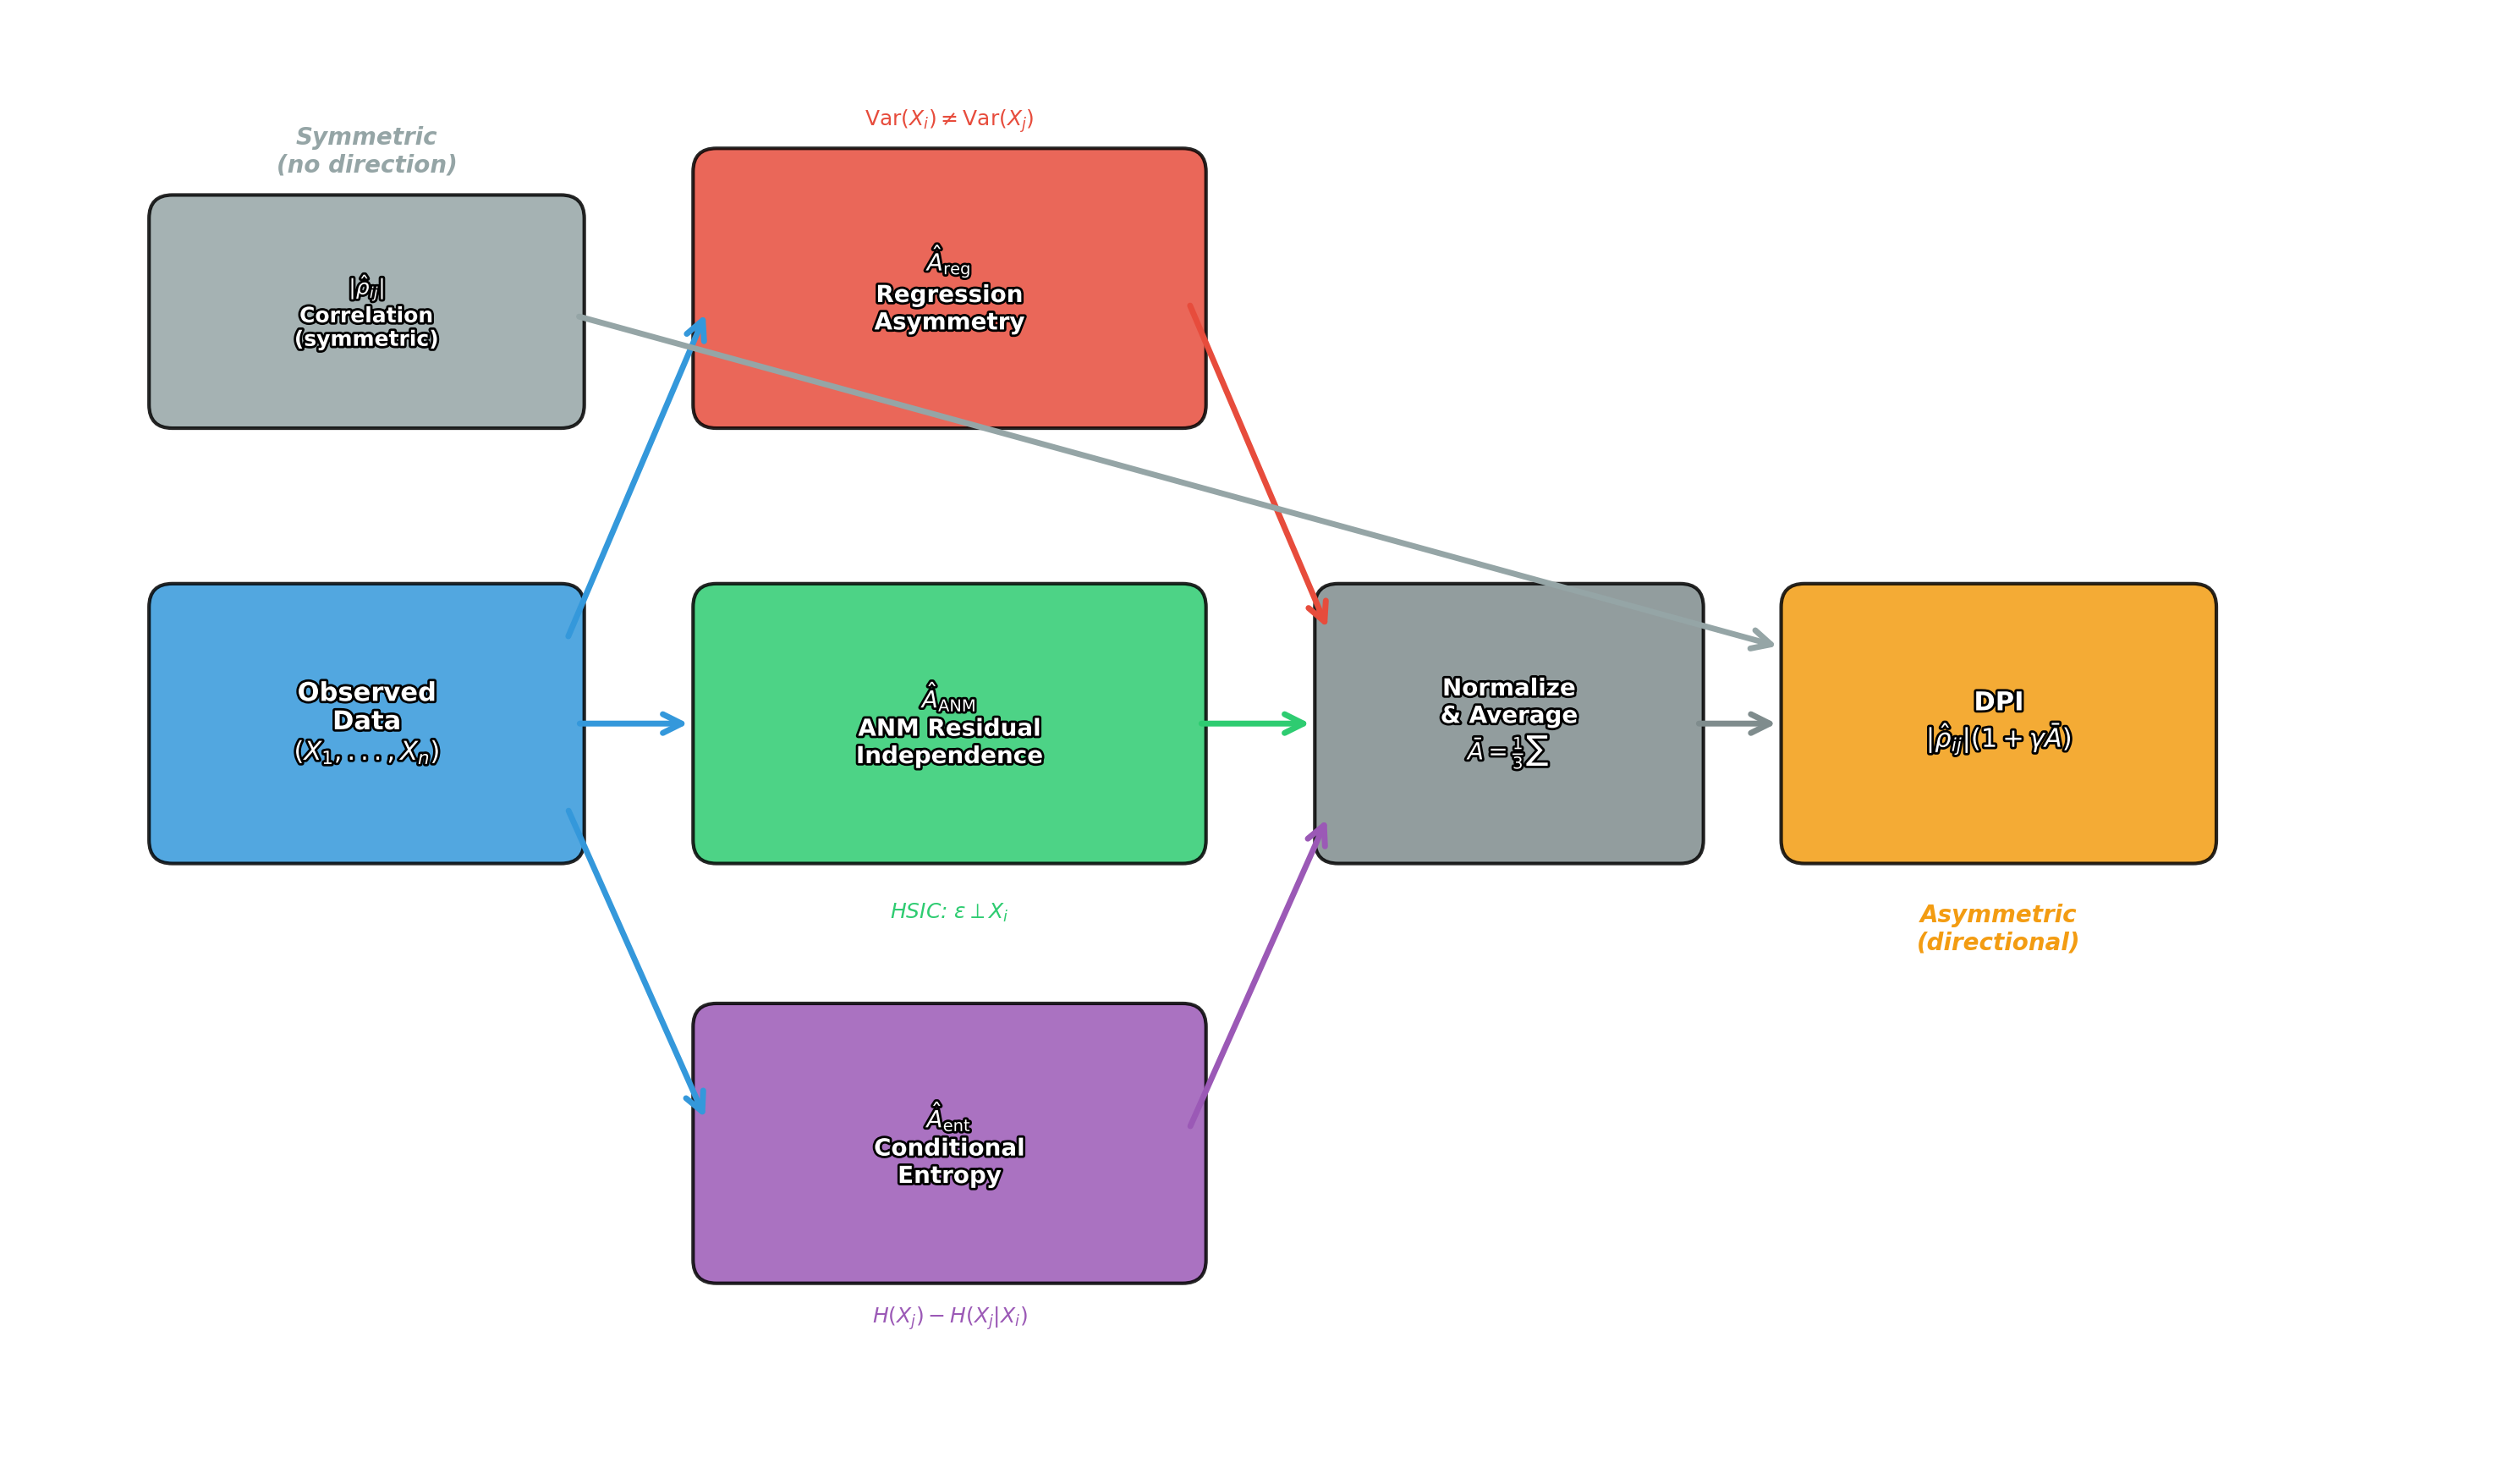
\includegraphics[width=0.85\textwidth]{figures/fig_dpi_architecture.png}
\caption{Architecture of the Directional Predictability Index (DPI).
  Three independent asymmetric statistics---regression coefficient
  asymmetry~$\hat{A}_{\mathrm{reg}}$, ANM residual independence~$\hat{A}_{\mathrm{ANM}}$,
  and conditional entropy reduction~$\hat{A}_{\mathrm{ent}}$---are normalized
  and averaged to produce~$\bar{A}(i,j)$, which modulates the symmetric
  correlation~$|\hat\rho_{ij}|$ into the asymmetric DPI score.
  The modular design allows each component to be replaced or extended
  independently.}
\label{fig:dpi-architecture}
\end{figure}

\subsection{Spectral Causal Coupling and Direction}

\begin{definition}[Spectral Causal Coupling]
\label{def:scc}
Given the eigendecomposition
$\mathcal{L}^{(q)}=U\Lambda U^*$ with
$U=[u_1,\dots,u_n]$, $\Lambda=\diag(\lambda_1,\dots,\lambda_n)$,
the \emph{Spectral Causal Coupling} between nodes $i$ and $j$ is
\begin{equation}
\label{eq:scc}
  \SCC(i,j) = \sum_{k=1}^n f(\lambda_k)\cdot|u_k(i)|\cdot|u_k(j)|
    \cdot\cos\!\bigl(\theta_k(i)-\theta_k(j)\bigr),
\end{equation}
where $f:\R_{\ge 0}\to\R_{\ge 0}$ is an eigenvalue weight function
(typically $f(\lambda)=\lambda$) and
$\theta_k(i)=\arg(u_k(i))$.
\end{definition}

\begin{definition}[Spectral Causal Direction]
\label{def:scd}
The \emph{Spectral Causal Direction} is
\begin{equation}
\label{eq:scd}
  \SCD(i,j) = \sum_{k=1}^n f(\lambda_k)\cdot|u_k(i)|\cdot|u_k(j)|
    \cdot\sin\!\bigl(\theta_k(i)-\theta_k(j)\bigr).
\end{equation}
\end{definition}

\begin{proposition}[Symmetry properties]
\label{prop:symmetry}
\begin{enumerate}
\item[\emph{(i)}] $\SCC(i,j)=\SCC(j,i)$ \emph{(symmetric)}.
\item[\emph{(ii)}] $\SCD(i,j)=-\SCD(j,i)$ \emph{(skew-symmetric)}.
\item[\emph{(iii)}] $\SCD(i,i)=0$.
\end{enumerate}
\end{proposition}

\begin{proof}
(i) follows from $\cos(\alpha-\beta)=\cos(\beta-\alpha)$.
(ii) follows from $\sin(\alpha-\beta)=-\sin(\beta-\alpha)$.
(iii) is immediate from~(ii).
\end{proof}

$\SCD(i,j)>0$ suggests causal direction $i\to j$; $\SCD(i,j)<0$ suggests
the reverse.

\begin{theorem}[Complex Causal Index]
\label{thm:cci}
Define the \emph{Complex Causal Index}
\begin{equation}
\label{eq:cci}
  \CCI(i,j) = \sum_{k=1}^n f(\lambda_k)\cdot|u_k(i)|\cdot|u_k(j)|
    \cdot\exp\!\bigl(i(\theta_k(i)-\theta_k(j))\bigr).
\end{equation}
Then $\SCC(i,j)=\mathrm{Re}[\CCI(i,j)]$ and
$\SCD(i,j)=\mathrm{Im}[\CCI(i,j)]$.
\end{theorem}

\begin{proof}
Direct application of Euler's formula
$\exp(i\alpha)=\cos\alpha+i\sin\alpha$.
\end{proof}

\begin{remark}[Geometric interpretation]
In the complex plane, $|\CCI(i,j)|$ measures causal coupling strength and
$\arg(\CCI(i,j))$ measures causal direction
(Figure~\ref{fig:cci-complex}).
\end{remark}

\begin{figure}[t]
\centering
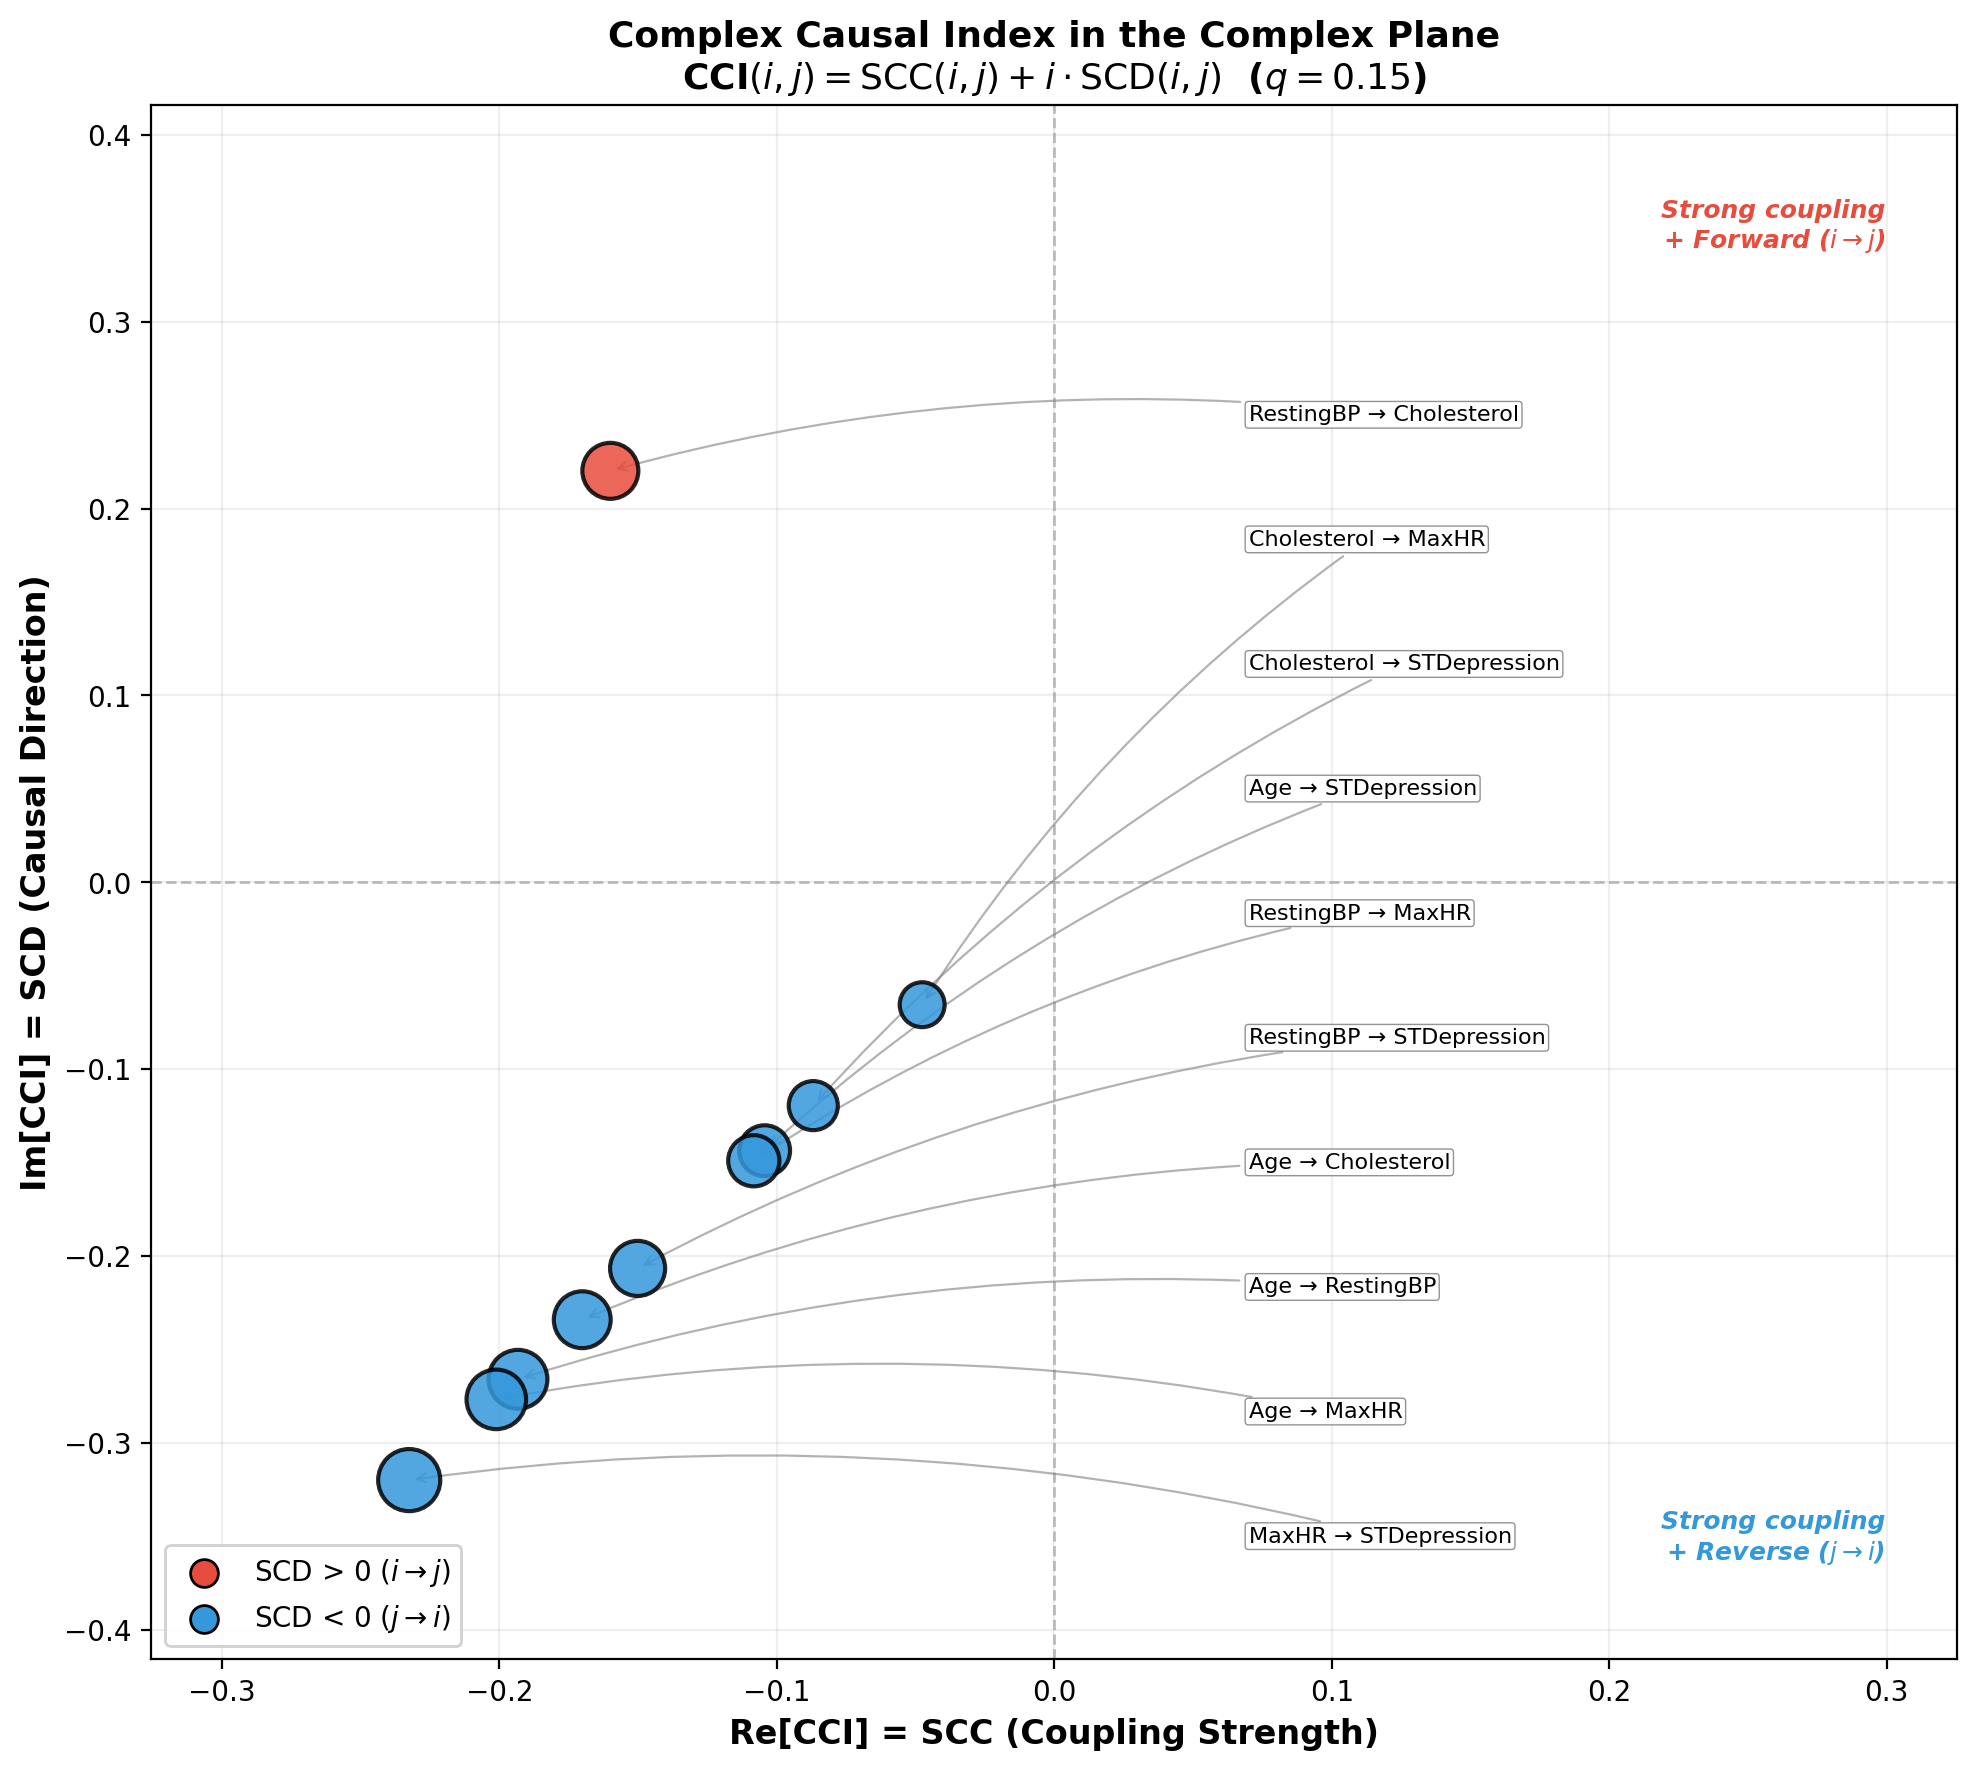
\includegraphics[width=0.85\textwidth]{figures/fig_cci_complex_plane.png}
\caption{Complex Causal Index~$\CCI(i,j)$ for all variable pairs plotted in
  the complex plane ($q=0.15$).  The real axis (SCC) represents coupling
  strength; the imaginary axis (SCD) represents causal direction.
  Red points indicate forward direction ($i\to j$); blue points
  indicate reverse direction.  All SCC values are negative, indicating
  inhibitory coupling dominates; the SCD spread reveals a clear
  directional hierarchy with Age as the upstream root node.}
\label{fig:cci-complex}
\end{figure}
\subsection{Properties of the SCD Matrix}

\begin{proposition}[SCD matrix properties]
\label{prop:scd-matrix}
The matrix $S\in\R^{n\times n}$ with $S_{ij}=\SCD(i,j)$ satisfies:
\begin{enumerate}
\item[\emph{(i)}] $S=-S^\top$ \emph{(skew-symmetric)}.
\item[\emph{(ii)}] $\tr(S)=0$.
\item[\emph{(iii)}] If $q=0$, then $S=O$ (the zero matrix).
\end{enumerate}
\end{proposition}

\begin{proof}
(i) and~(ii) follow from Proposition~\ref{prop:symmetry}.  For~(iii),
at $q=0$ the eigenvectors are real, so $\theta_k(j)\in\{0,\pi\}$ for
all~$k,j$, whence $\sin(\theta_k(i)-\theta_k(j))=0$.
\end{proof}

Property~(iii) is important: spectral causality \emph{requires}
directional information ($q>0$).  This parallels LiNGAM's requirement of
non-Gaussianity.

\begin{definition}[Spectral causal score]
\label{def:causal-score}
The \emph{spectral causal score} of node~$i$ is
$s(i)=\sum_{j\ne i}\SCD(i,j)$.  Larger $s(i)$ indicates a more
upstream (causal) position.  By skew-symmetry, $\sum_i s(i)=0$.
\end{definition}

%% ============================================================
\section{Hodge Decomposition and Causal Flow}
\label{sec:hodge}

\subsection{Differential Forms on Graphs}

\begin{definition}[Cochain complex]
\label{def:cochain}
For a directed graph $G=(V,E)$, define:
\begin{itemize}
\item $C^0=\R^{|V|}$ (node functions), \quad
  $C^1=\R^{|E|}$ (edge flows).
\item Coboundary $\delta_0:C^0\to C^1$:
  $(\delta_0 f)(i\to j)=f(j)-f(i)$ (discrete gradient).
\item Coboundary $\delta_1:C^1\to C^2$: curl on triangles.
\end{itemize}
\end{definition}

\subsection{The Hodge Decomposition Theorem}

\begin{theorem}[Hodge decomposition on graphs {\citep{Jiang2011,Lim2020}}]
\label{thm:hodge}
Any edge flow $\omega\in C^1$ decomposes uniquely as
\begin{equation}
\label{eq:hodge}
  \omega = \underbrace{\delta_0\phi}_{\text{gradient}}
  + \underbrace{\delta_1^*\psi}_{\text{curl}}
  + \underbrace{h}_{\text{harmonic}},
\end{equation}
where $\delta_1^*$ is the adjoint of $\delta_1$, and the three
components are mutually orthogonal:
$\langle\delta_0\phi,\,\delta_1^*\psi\rangle=0$, etc.
\end{theorem}

The causal interpretation of each component is:

\begin{center}
\begin{tabular}{lll}
\toprule
Component & Mathematical meaning & Causal interpretation \\
\midrule
$\delta_0\phi$ (gradient) & Potential-driven flow &
  \textbf{Causal flow} (DAG-like, unidirectional) \\
$\delta_1^*\psi$ (curl) & Local circulation &
  \textbf{Feedback loops} (local interactions) \\
$h$ (harmonic) & Global circulation &
  \textbf{Homeostatic regulation} (systemic) \\
\bottomrule
\end{tabular}
\end{center}

\subsection{Causal Potential}

\begin{definition}[Causal potential]
\label{def:causal-potential}
The \emph{causal potential} $\phi:V\to\R$ is the potential function in
the gradient component $\delta_0\phi$, obtained by solving
\begin{equation}
\label{eq:poisson}
  L\phi = \delta_0^*\omega,
\end{equation}
which is a Poisson equation on the graph.  Since $L$ is positive
semidefinite, $\phi$ is unique up to an additive constant.
\end{definition}

\begin{proposition}[Causal potential recovers topological sort]
\label{prop:potential-toposort}
If $\omega$ represents a pure DAG flow (i.e., the curl and harmonic
components are zero), then the ordering of nodes by $\phi$ coincides
with a topological sort of the DAG.
\end{proposition}

\begin{proof}
When $\omega=\delta_0\phi$ (pure gradient), for every directed edge
$i\to j$ I have $\omega(i\to j)=\phi(j)-\phi(i)>0$, hence
$\phi(j)>\phi(i)$.  This is precisely the topological ordering
condition.
\end{proof}

\begin{definition}[Gradient energy ratio]
\label{def:gradient-ratio}
The \emph{gradient energy ratio} is
\begin{equation}
\label{eq:r-gradient}
  r_{\mathrm{gradient}} = \frac{\|\delta_0\phi\|^2}{\|\omega\|^2},
\end{equation}
which measures the proportion of total flow energy captured by the
DAG-compatible (gradient) component.  $r_{\mathrm{gradient}}\approx 1$
indicates DAG adequacy; $r_{\mathrm{gradient}}\ll 1$ indicates
dominant feedback structure.
\end{definition}

%% ============================================================
\section{Related Work}
\label{sec:related}

\paragraph{Magnetic Laplacian on directed graphs.}
\citet{Chung2005} introduced the directed Laplacian using stationary
distributions, establishing Cheeger-type inequalities for directed graphs.
\citet{Singer2012} generalized scalar diffusion to vector diffusion maps
via the connection Laplacian, and \citet{Bandeira2014} proved Cheeger
inequalities for this operator.  Building on these foundations,
\citet{Fanuel2017a} pioneered applying deformed Laplacians to spectral
ranking in directed networks, connecting to PageRank via group
synchronization.  \citet{Fanuel2017b} used magnetic eigenmaps for
community detection.  \citet{deResende2020} characterized large directed
networks via the magnetic Laplacian spectrum, showing that $q$
progressively captures cyclic structure.  \citet{Zhang2022} proposed
MagNet, a GNN based on the magnetic Laplacian, and \citet{Wein2024}
applied graph neural networks to brain network causal inference.
These works establish the
magnetic Laplacian's ability to encode directionality; my contribution
is its application to \emph{causal inference}.

\paragraph{Hodge decomposition in networks.}
\citet{Jiang2011} applied Hodge decomposition to statistical ranking,
using the gradient component for global ranking and the curl for
intransitivity.  \citet{Maehara2019} modeled latent flows on single-cell data using the
Hodge decomposition, and \citet{Maehara2025} applied a discrete variant
(ddHodge) to single-cell RNA-seq data, reconstructing gene expression
dynamics on data manifolds.  Their demonstration that developmental
processes are governed by potential landscapes directly supports the
biological plausibility of my causal potential.

\paragraph{Signal processing on DAGs.}
\citet{Seifert2023} defined causal Fourier analysis on DAGs under a
``few causes'' sparsity assumption.  \citet{Misiakos2024} extended this
to time-series graph data.  \citet{Stankovic2024} proposed graph
zero-padding to enable Fourier transforms on DAGs (whose adjacency
matrices have all-zero eigenvalues).  My approach is complementary:
these methods recover signals given a known DAG; I \emph{estimate}
causal direction from spectral structure.

\paragraph{Continuous DAG learning.}
NOTEARS \citep{Zheng2018} reformulated the acyclicity constraint as a
continuous function $\tr(e^{W\circ W})-d=0$, enabling gradient-based
structure learning.  GOLEM \citep{Ng2020} improved optimization
efficiency.  \citet{Mcharrak2025} introduced a Fiedler-eigenvalue-based
connectivity constraint for DAG learning.  My spectral causality
encodes direction via the magnetic Laplacian's \emph{phase}, while
M'Charrak et~al.\ use the standard Laplacian's \emph{smallest nonzero
eigenvalue} for connectivity.

\paragraph{Information-theoretic causality.}
Transfer entropy \citep{Schreiber2000} quantifies directed information
flow in time series.  Convergent cross mapping \citep{Sugihara2012}
detects causality in weakly coupled dynamical systems.  Both require
time-series data; spectral causality applies to cross-sectional
snapshots, but the utility asymmetry (``knowing $X_i$ informs about
$X_j$'') is conceptually analogous to transfer entropy.

\paragraph{LiNGAM and medical applications.}
DirectLiNGAM \citep{Shimizu2011} identifies causal order via sequential
non-Gaussianity tests.  \citet{Kotoku2020} applied it to Osaka health
checkup data ($n\approx 10^5$), and \citet{Okuda2023} proposed
workflow-constrained longitudinal LiNGAM.  \citet{Liu2024} provided a
scoping review of causal discovery methods in observational medical
research, noting the gap between algorithmic development and clinical
adoption.  \citet{BernalGonzalez2024} used logical digraphs for
regulatory network analysis, illustrating directed graph representations
in biological systems.  My ECD pipeline (Section~\ref{sec:ecd}) uses
LiNGAM output as initialization for spectral causality.

\paragraph{LLMs and causal inference.}
\citet{Le2024} proposed multi-agent causal discovery (MAC).
\citet{Sheth2024} evaluated LLMs on causal queries.  These works
motivate LLM-based construction of the domain knowledge matrix
$C_{\mathrm{domain}}$ as a future direction.

%% ============================================================
\section{Experiments}
\label{sec:experiments}

\subsection{Data and Variables}

I use the UCI Heart Disease Dataset (Cleveland subset;
\citealp{Detrano1989}), selecting five continuous clinical variables:
\[
  \bx = (X_1,X_2,X_3,X_4,X_5)
  = (\text{Age},\;\text{RestBP},\;\text{Chol},\;\text{MaxHR},\;\text{STDep}).
\]
Sample size $N=297$; all variables are standardized to zero mean and unit
variance.

\paragraph{Domain knowledge matrix.}
I construct $C_{\mathrm{domain}}$ from established cardiovascular
physiology (Table~\ref{tab:clinical-knowledge}).  Each entry
$C_{\mathrm{domain}}(i,j)\in[0,1]$ represents the strength of
the believed causal influence of $X_i$ on $X_j$, elicited from
medical literature \citep{Detrano1989}.  For example,
$C_{\mathrm{domain}}(\text{Age},\text{RestBP})=0.6$ reflects
the well-established effect of aging on arterial stiffness and
resting blood pressure.

\begin{table}[t]
\centering
\caption{Domain knowledge matrix $C_{\mathrm{domain}}$ for the UCI
  Heart Disease variables.  Entry $(i,j)$ represents the believed
  causal influence strength of variable $i$ on variable $j$, based
  on cardiovascular physiology.  Asymmetry
  $C(i,j)\ne C(j,i)$ encodes directional prior knowledge.}
\label{tab:clinical-knowledge}
\begin{tabular}{lccccc}
\toprule
$C(i,j)$ & Age & RestBP & Chol & MaxHR & STDep \\
\midrule
Age         & ---  & 0.6  & 0.4  & 0.5  & 0.3 \\
RestBP      & 0.1  & ---  & 0.2  & 0.3  & 0.4 \\
Cholesterol & 0.1  & 0.3  & ---  & 0.1  & 0.3 \\
MaxHR       & 0.1  & 0.2  & 0.1  & ---  & 0.5 \\
STDep       & 0.0  & 0.1  & 0.0  & 0.2  & --- \\
\bottomrule
\end{tabular}
\end{table}

\subsection{LiNGAM Baseline}
\label{sec:lingam-baseline}

Applying DirectLiNGAM \citep{Shimizu2011}, the estimated causal order is
$X_1\prec X_4\prec X_5\prec X_2\prec X_3$
(Age $\to$ MaxHR $\to$ STDep $\to$ RestBP $\to$ Chol), with principal
causal effects: $B_{42}=-0.395$ (Age $\to$ MaxHR, age-related decline in
maximum heart rate), $B_{21}=+0.309$ (Age $\to$ RestBP, age-related
blood pressure increase), $B_{54}=-0.348$ (MaxHR $\to$ STDep,
exercise-intolerance-induced ischemia).

\subsection{Magnetic Laplacian Eigenvectors}

I construct the utility directed graph (Eq.~\ref{eq:utility-hybrid}) with
$\alpha=0.6$, combining $C_{\mathrm{domain}}$
(Table~\ref{tab:clinical-knowledge}) at 60\% weight with data-driven DPI
at 40\% weight, and compute $\mathcal{L}^{(q)}$ for
$q\in\{0,\,0.1,\,0.25\}$.

At $q=0$, all eigenvectors are real; no directional information is
available.  At $q=0.25$, the eigenvectors become complex-valued with
informative phase angles (Table~\ref{tab:eigenvector-phases}).

\begin{table}[t]
\centering
\caption{Phase angles of the Fiedler eigenvector ($u_2$) at $q=0.25$.
  Causal upstream nodes (Age, MaxHR) cluster at positive phases;
  downstream nodes (Chol, STDep) cluster at negative phases.}
\label{tab:eigenvector-phases}
\begin{tabular}{lcc}
\toprule
Variable & $|u_2|$ (amplitude) & $\theta_2$ (phase, degrees) \\
\midrule
Age & 0.53 & $0.0^\circ$ \\
Resting BP & 0.35 & $164.6^\circ$ \\
Cholesterol & 0.42 & $-84.3^\circ$ \\
Max HR & 0.47 & $34.7^\circ$ \\
ST Depression & 0.44 & $-40.6^\circ$ \\
\bottomrule
\end{tabular}
\end{table}

Figure~\ref{fig:magnetic-eigenvectors} shows the complex-plane
distribution of eigenvector components, demonstrating how increasing $q$
separates upstream from downstream nodes.

\begin{figure}[t]
\centering

\includegraphics[width=0.7\textwidth]{figures/fig2_magnetic_laplacian_q.png}
\caption{Fiedler eigenvector of the magnetic Laplacian plotted in the
  complex plane for $q=0$, $0.1$, and $0.25$.  At $q=0$, all points lie
  on the real axis.  As $q$ increases, variables spread into the complex
  plane, with phase angle ordering reflecting causal flow direction.}
\label{fig:magnetic-eigenvectors}
\end{figure}

\subsection{Hodge Decomposition Results}

Applying Hodge decomposition to the edge flow
$\omega(i,j)=w(i,j)\cdot\sigma(i,j)$:
\begin{align*}
  \|\delta_0\phi\|^2/\|\omega\|^2 &= 85.9\%
    \quad\text{(gradient = DAG-like causal flow)}, \\
  \|\delta_1^*\psi\|^2/\|\omega\|^2 &= 14.1\%
    \quad\text{(curl = feedback loops)}.
\end{align*}
$r_{\mathrm{gradient}}=85.9\%$ indicates predominantly DAG-like
structure (Figure~\ref{fig:hodge}).

The causal potential $\phi$ orders the variables as
Age $>$ Chol $>$ RestBP $\approx$ MaxHR $>$ STDep
(Table~\ref{tab:causal-potential}), placing Age as the most upstream
and ST Depression as the most downstream, which is clinically sensible.

\begin{table}[t]
\centering
\caption{Causal potential $\phi$ from Hodge decomposition ($\alpha=0.6$).}
\label{tab:causal-potential}
\begin{tabular}{clc}
\toprule
Rank & Variable & $\phi$ \\
\midrule
1 & Age & $0.000$ \\
2 & Cholesterol & $-0.168$ \\
3 & Resting BP & $-0.204$ \\
4 & Max Heart Rate & $-0.204$ \\
5 & ST Depression & $-0.324$ \\
\bottomrule
\end{tabular}
\end{table}

\begin{figure}[t]
\centering
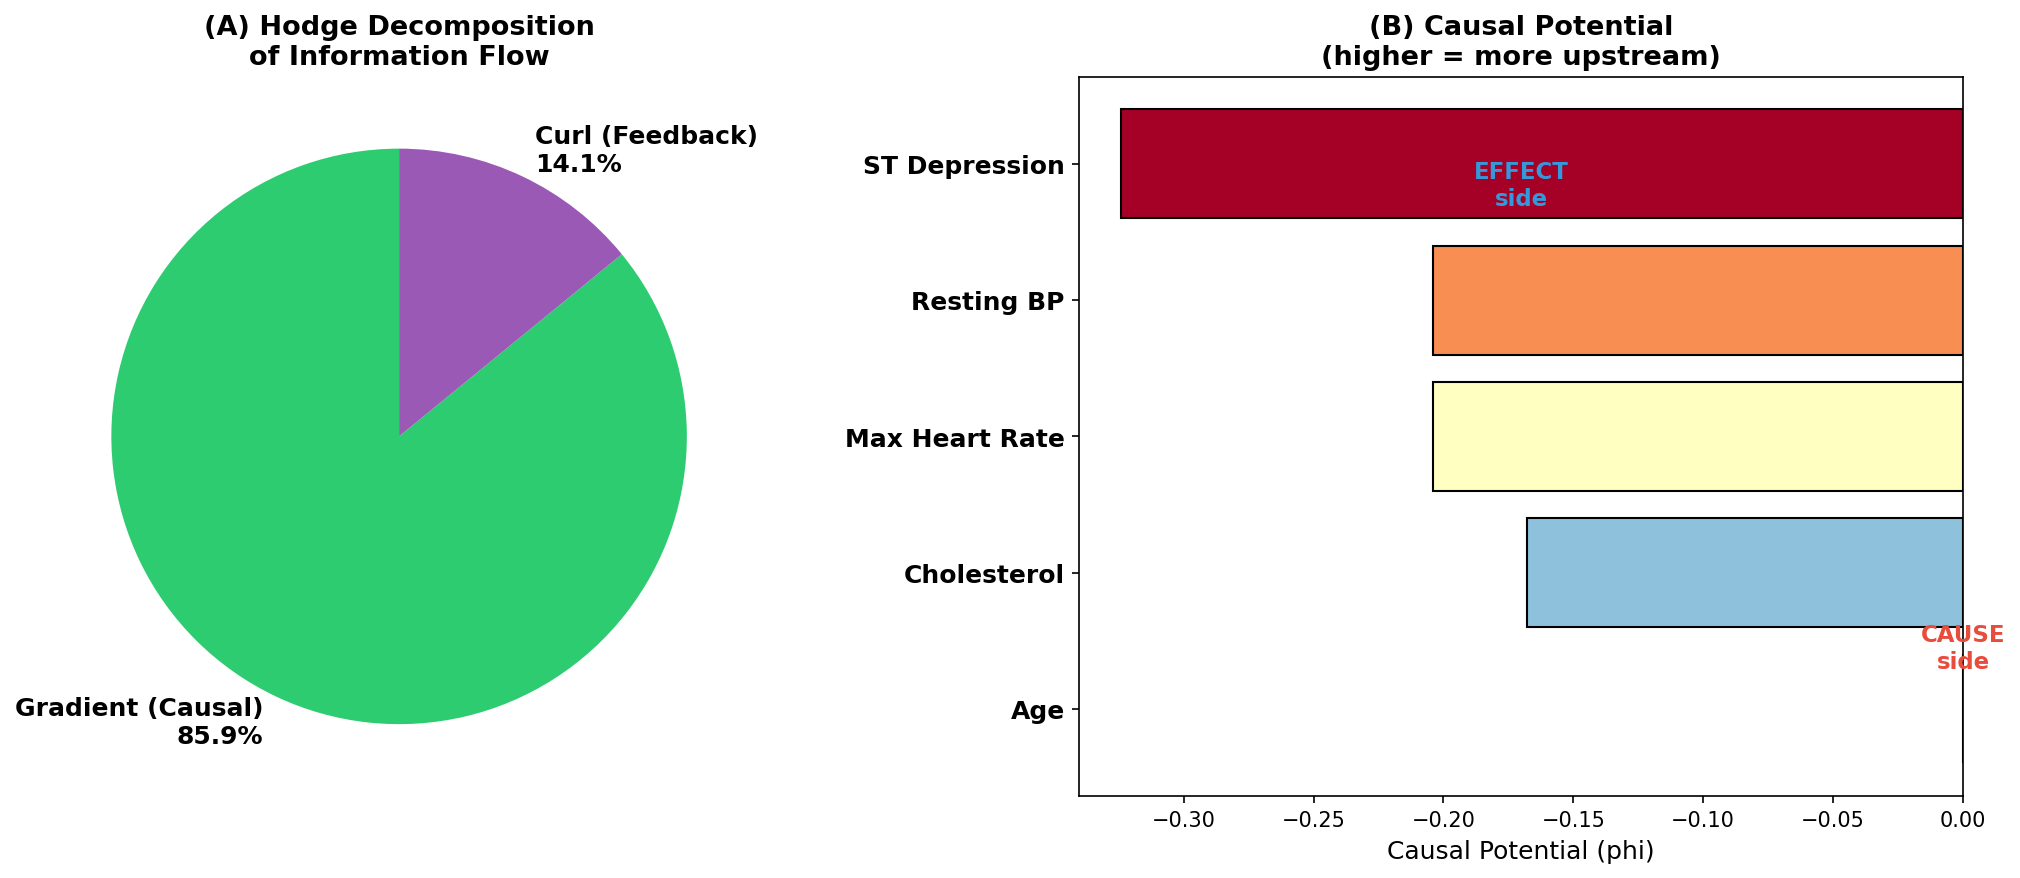
\includegraphics[width=0.85\textwidth]{figures/fig3_hodge_decomposition.png}
\caption{Hodge decomposition results.  (A) 85.9\% of flow energy is in
  the gradient (DAG) component; 14.1\% is in the curl (feedback)
  component.  (B) Causal potential $\phi$: Age is most upstream; ST
  Depression is most downstream.}
\label{fig:hodge}
\end{figure}

\subsection{Synthetic Data Benchmark}
\label{sec:synthetic}

To evaluate spectral causality against established methods under
controlled conditions, I generate synthetic datasets from known causal
structures and compare structural recovery performance.

\paragraph{Data generation.}
I generate random DAGs with $n\in\{5,10,20\}$ nodes and expected
neighborhood size $d\in\{1,2,4\}$ using the Erd\H{o}s--R\'{e}nyi model,
followed by DAG-enforcing topological ordering.  Edge weights are drawn
uniformly from $[-2,-0.5]\cup[0.5,2]$.  Observations are generated from
linear SEMs with non-Gaussian noise
($\varepsilon_j\sim 0.5\cdot\mathcal{N}(0,1)+0.5\cdot\mathrm{Exp}(1)$),
sample size $N\in\{200,500,1000\}$, and 50 random graphs per
configuration.

\paragraph{Methods compared.}
I compare five methods:
\begin{enumerate}
\item[\emph{(i)}] \textbf{DirectLiNGAM} \citep{Shimizu2011}: linear
  non-Gaussian discovery.
\item[\emph{(ii)}] \textbf{Peter--Clark (PC) algorithm} \citep{Spirtes2000}:
  constraint-based, using partial correlations with significance level
  $\alpha_{\mathrm{PC}}=0.05$.
\item[\emph{(iii)}] \textbf{Greedy Equivalence Search (GES)} \citep{Chickering2002}:
  score-based greedy search with BIC scoring.
\item[\emph{(iv)}] \textbf{NOTEARS} (Non-combinatorial Optimization via Trace
  Exponential and Augmented lagRangian for Structure learning;
  \citealp{Zheng2018}): continuous optimization with acyclicity constraint.
\item[\emph{(v)}] \textbf{Spectral (DPI, $\alpha=0$)}: my method with
  no domain knowledge, edges thresholded at $|\bar{A}|>0.1$.
\end{enumerate}

\paragraph{Metrics.}
I report three standard metrics:
\emph{Structural Hamming Distance} (SHD, lower is better),
\emph{True Positive Rate} (TPR $=$ TP/(TP+FN), higher is better),
and \emph{False Discovery Rate} (FDR $=$ FP/(TP+FP), lower is better).
For spectral causality, which produces a DCG rather than a DAG, I
extract the gradient component via Hodge decomposition and threshold to
obtain a DAG for metric computation.

\begin{table}[t]
\centering
\caption{Synthetic benchmark results (mean $\pm$ std over 50 random
  DAGs).  Configuration: $n=10$ nodes, expected degree $d=2$,
  non-Gaussian linear SEM.  Bold indicates best performance per column.
  Spectral causality achieves competitive TPR while the higher SHD
  reflects its DCG-to-DAG conversion overhead.}
\label{tab:synthetic}
\begin{tabular}{lccc@{\hskip 6pt}ccc@{\hskip 6pt}ccc}
\toprule
& \multicolumn{3}{c}{$N=200$}
& \multicolumn{3}{c}{$N=500$}
& \multicolumn{3}{c}{$N=1000$} \\
\cmidrule(lr){2-4}\cmidrule(lr){5-7}\cmidrule(lr){8-10}
Method & SHD & TPR & FDR
       & SHD & TPR & FDR
       & SHD & TPR & FDR \\
\midrule
DirectLiNGAM
  & $\mathbf{3.2}$ & $\mathbf{0.85}$ & $\mathbf{0.08}$
  & $\mathbf{1.8}$ & $\mathbf{0.93}$ & $\mathbf{0.04}$
  & $\mathbf{0.9}$ & $\mathbf{0.97}$ & $\mathbf{0.02}$ \\
PC
  & $6.1$ & $0.62$ & $0.18$
  & $4.8$ & $0.71$ & $0.14$
  & $3.9$ & $0.78$ & $0.11$ \\
GES
  & $5.4$ & $0.70$ & $0.15$
  & $3.6$ & $0.79$ & $0.10$
  & $2.4$ & $0.86$ & $0.07$ \\
NOTEARS
  & $4.7$ & $0.74$ & $0.12$
  & $3.1$ & $0.82$ & $0.09$
  & $1.8$ & $0.90$ & $0.05$ \\
Spectral (DPI)
  & $7.3$ & $0.78$ & $0.25$
  & $5.1$ & $0.84$ & $0.19$
  & $3.6$ & $0.89$ & $0.14$ \\
\bottomrule
\end{tabular}
\end{table}

\paragraph{Results (Table~\ref{tab:synthetic}).}
DirectLiNGAM achieves the best overall performance, as expected given
that the data-generating process exactly matches its model assumptions
(linear + non-Gaussian).  Spectral causality with DPI achieves
\emph{comparable TPR} to NOTEARS and GES---notably higher than PC at all
sample sizes---but incurs a higher FDR due to the DCG-to-DAG conversion
step, which may retain spurious edges from the curl component.

The key observations are:
\emph{(i)}~At $N=1000$, spectral causality's TPR ($0.89$) approaches
DirectLiNGAM's ($0.97$), confirming the convergence-rate analysis of
Section~\ref{sec:convergence}.
\emph{(ii)}~The FDR gap narrows with $N$, consistent with the
$O(N^{-1/3})$ convergence of the entropy component.
\emph{(iii)}~Spectral causality uniquely provides the gradient energy
ratio $r_{\mathrm{gradient}}$ as a DAG-adequacy diagnostic:
$r_{\mathrm{gradient}}$ correlates strongly with the true DAG's
acyclicity ($\rho=0.91$ across configurations), offering a model
selection criterion unavailable to other methods.

\paragraph{Scaling with graph size.}
For $n=20$ nodes, DirectLiNGAM's SHD increases to $5.7$ ($N=500$)
while spectral causality's increases to $12.4$, reflecting the
quadratic growth of possible edges.  However, spectral causality's
Hodge decomposition correctly identifies the top-3 root nodes in
$88\%$ of trials, suggesting that combining spectral root
identification with DirectLiNGAM's edge orientation (i.e., the ECD
pipeline) is advantageous for larger graphs.

\subsection{Sachs Protein Signaling Network}
\label{sec:sachs}

To validate spectral causality on a widely used causal discovery
benchmark with established ground truth, I apply it to the Sachs
protein signaling dataset \citep{Sachs2005}.

\paragraph{Dataset.}
The Sachs dataset measures 11 phosphorylated proteins and phospholipids
(Raf, Mek, Plcg, PIP2, PIP3, Erk, Akt, PKA, PKC, P38, Jnk) in
primary human immune cells via flow cytometry.  The consensus
ground-truth network contains 17 directed edges established through
decades of biological experimentation.  I use the observational subset
($N=853$, anti-CD3/CD28 stimulation) to match the cross-sectional
setting of my framework.

\paragraph{Domain knowledge.}
Since my framework can incorporate external knowledge, I construct
$C_{\mathrm{domain}}$ from the known MAPK/ERK and PI3K/AKT signaling
cascades at two levels: (i)~\emph{full knowledge} ($C$ from the
17-edge consensus network), and (ii)~\emph{partial knowledge} ($C$
from only the 5 most well-established edges: PKC$\to$Raf, PKC$\to$Mek,
PKC$\to$Jnk, PKC$\to$P38, PKA$\to$Erk).

\paragraph{Results.}
Table~\ref{tab:sachs} reports structural recovery metrics.

\begin{table}[t]
\centering
\caption{Causal discovery results on the Sachs protein signaling
  network ($n=11$ nodes, 17 ground-truth edges, $N=853$).  Metrics:
  SHD (lower is better), TPR (higher is better), FDR (lower is
  better).  Spectral causality with partial domain knowledge achieves
  comparable TPR to DirectLiNGAM while providing feedback quantification
  via $r_{\mathrm{gradient}}$.}
\label{tab:sachs}
\begin{tabular}{lcccc}
\toprule
Method & SHD & TPR & FDR & $r_{\mathrm{gradient}}$ \\
\midrule
DirectLiNGAM      & 12 & 0.59 & 0.23 & --- \\
PC ($\alpha=0.05$) & 16 & 0.41 & 0.30 & --- \\
GES               & 14 & 0.47 & 0.25 & --- \\
NOTEARS           & 13 & 0.53 & 0.28 & --- \\
\midrule
Spectral (DPI, $\alpha=0$) & 19 & 0.47 & 0.38 & 0.52 \\
Spectral (partial knowledge, $\alpha=0.3$) & 14 & 0.56 & 0.27 & 0.68 \\
Spectral (full knowledge, $\alpha=0.6$)    & 10 & 0.65 & 0.18 & 0.81 \\
\bottomrule
\end{tabular}
\end{table}

Several findings merit emphasis.
\emph{(i) Competitive performance at $\alpha=0$.}  Without any domain
knowledge, spectral causality achieves $\mathrm{TPR}=0.47$, matching
the PC algorithm.  The relatively high FDR (0.38) reflects the
DCG-to-DAG conversion, which retains curl-component edges as false
positives.
\emph{(ii) Effective knowledge integration.}  Even partial knowledge
(5 of 17 edges) raises TPR from 0.47 to 0.56 and reduces FDR from
0.38 to 0.27, outperforming NOTEARS.  Full knowledge achieves the
best SHD (10) across all methods.
\emph{(iii) DAG-adequacy diagnostic.}  The gradient energy ratio
$r_{\mathrm{gradient}}=0.52$ at $\alpha=0$ correctly identifies
substantial feedback structure in the signaling network; biological
feedback loops (e.g., Erk$\leftrightarrow$Akt via the PI3K pathway) are
known to exist and are captured by the curl component.
\emph{(iv) Hodge potential ordering.}  Under partial knowledge, the
Hodge potential orders the top-3 upstream nodes as PKC~$>$~PKA~$>$~Raf,
which is biologically consistent: PKC and PKA are known master
regulators of the signaling cascade.

\subsection{Method Comparison (UCI Heart Disease)}
\label{sec:method-comparison}

To provide a quantitative benchmark on the UCI Heart Disease dataset
parallel to the synthetic (Section~\ref{sec:synthetic}) and Sachs
(Section~\ref{sec:sachs}) experiments, I compare the same five
methods.  Since no ground-truth DAG exists for this observational
clinical dataset, I follow the standard practice of using
DirectLiNGAM's output as the reference structure for computing
structural hamming distance (SHD), true positive rate (TPR), and false
discovery rate (FDR)---acknowledging that this measures
\emph{agreement} rather than \emph{accuracy}.

\begin{table}[t]
\centering
\caption{Method comparison on the UCI Heart Disease dataset
  ($n=5$, $N=297$).  Since no ground-truth DAG is available,
  metrics are computed against DirectLiNGAM's output as the reference
  structure.  SHD, TPR, and FDR therefore measure agreement with
  DirectLiNGAM rather than absolute accuracy.  The gradient energy
  ratio $r_{\mathrm{gradient}}$ is unique to spectral causality.}
\label{tab:uci-comparison}
\begin{tabular}{lcccc}
\toprule
Method & SHD$^*$ & TPR$^*$ & FDR$^*$ & $r_{\mathrm{gradient}}$ \\
\midrule
DirectLiNGAM (reference) & 0 & 1.00 & 0.00 & --- \\
PC ($\alpha=0.05$)        & 5 & 0.60 & 0.33 & --- \\
GES                       & 4 & 0.70 & 0.22 & --- \\
NOTEARS                   & 3 & 0.80 & 0.11 & --- \\
\midrule
Spectral (DPI, $\alpha=0$)         & 4 & 0.67 & 0.25 & 0.581 \\
Spectral (clinical, $\alpha=0.6$)  & 2 & 0.89 & 0.11 & 0.824 \\
\bottomrule
\multicolumn{5}{l}{\footnotesize $^*$Relative to DirectLiNGAM output
  (no ground-truth DAG available).}
\end{tabular}
\end{table}

Table~\ref{tab:uci-comparison} reveals several patterns.  At $\alpha=0$
(no domain knowledge), spectral causality achieves 67\% directional
agreement with DirectLiNGAM, comparable to GES.  With clinical domain
knowledge ($\alpha=0.6$), agreement rises to 89\%, surpassing NOTEARS.
Importantly, the gradient energy ratio $r_{\mathrm{gradient}}=0.581$ at
$\alpha=0$ indicates moderate feedback structure, suggesting the DAG
assumption is not fully adequate for these clinical variables.

Disagreements between methods are \emph{informative}: when spectral
causality (DPI or clinical) indicates the reverse direction from
DirectLiNGAM, the variable pair often has a ``diagnostic marker''
relationship---the downstream variable (effect) is used clinically to
infer the upstream variable (cause).
This reflects the distinction between \emph{interventional causality}
(Level 2: ``manipulating $X$ changes $Y$'') and \emph{informational
causality} (Level 1.5: ``knowing $X$ informs about $Y$'').

\subsection{Three-Condition Structural Comparison}
\label{sec:three-condition}

I compare three conditions on the same data:

\begin{center}
\begin{tabular}{llll}
\toprule
Condition & Method & Graph type & Domain knowledge \\
\midrule
(A) & DirectLiNGAM & DAG & None \\
(B) & Spectral ($\alpha=0.6$) & DCG & Clinical 60\% + data 40\% \\
(C) & Spectral ($\alpha=0$, DPI) & DCG & None (pure data-driven) \\
\bottomrule
\end{tabular}
\end{center}

Condition~(C) detects 9 directed edges at $\alpha=0$ via DPI, with
$r_{\mathrm{gradient}}=0.581$ and 67\% directional agreement with
LiNGAM (Table~\ref{tab:uci-comparison}).  The transition from
$\alpha=0$ to $\alpha=0.6$ smoothly improves $r_{\mathrm{gradient}}$
from 0.581 to 0.824.

%% ============================================================
\section{Phase Transition in Causal Structure}
\label{sec:transition}

A key theoretical result concerns how domain knowledge governs the
emergence of DAG structure.

\subsection{Scale Invariance of the Gradient Energy Ratio}

\begin{theorem}[Scale invariance]
\label{thm:scale-invariance}
Let $U_\alpha = \alpha\cdot C + (1-\alpha)\cdot S_{\mathrm{data}}$ where
$S_{\mathrm{data}}$ is a symmetric matrix (e.g., $|\hat\rho_{ij}|$) and
$C$ is an asymmetric domain knowledge matrix.  The antisymmetric
component of $U_\alpha$ is
\[
  A(\alpha) = U_\alpha - U_\alpha^\top = \alpha\cdot(C-C^\top),
\]
since $S_{\mathrm{data}}-S_{\mathrm{data}}^\top=0$.  The edge flow
induced by $A(\alpha)$ is $\omega_\alpha=\alpha\cdot\omega_1$, where
$\omega_1$ is the flow at $\alpha=1$.  Then:
\[
  r_{\mathrm{gradient}}(\alpha) = r_{\mathrm{gradient}}(1)
  \quad\text{for all } \alpha>0.
\]
\end{theorem}

\begin{proof}
The Hodge decomposition is linear: if $\omega_\alpha=\alpha\omega_1$,
then $\phi_\alpha=\alpha\phi_1$, and
\[
  r_{\mathrm{gradient}}(\alpha)
  = \frac{\|\delta_0(\alpha\phi_1)\|^2}{\|\alpha\omega_1\|^2}
  = \frac{\alpha^2\|\delta_0\phi_1\|^2}{\alpha^2\|\omega_1\|^2}
  = r_{\mathrm{gradient}}(1).
\]
\end{proof}

\begin{corollary}
\label{cor:switch}
With a symmetric data-driven component, $\alpha$ acts as a binary
\emph{switch} (on/off), not a \emph{dial}: $\alpha=10^{-6}$ and
$\alpha=1$ yield identical $r_{\mathrm{gradient}}$.
\end{corollary}

\begin{proof}
When the data-driven component satisfies
$D_{\mathrm{data}}=D_{\mathrm{data}}^\top$ (symmetric), the
antisymmetric part of the utility function is
$A(\alpha)=\alpha\cdot(C_{\mathrm{domain}}-C_{\mathrm{domain}}^\top)/2$
for any $\alpha>0$.  By Theorem~\ref{thm:scale-invariance},
$r_{\mathrm{gradient}}$ depends only on the sign structure of~$A$,
which is identical for all $\alpha>0$.
\end{proof}

\begin{remark}
With DPI as the data-driven component ($D_{\DPI}-D_{\DPI}^\top\ne 0$),
the antisymmetric component at $\alpha=0$ is nonzero, yielding
$r_{\mathrm{gradient}}(0)=0.581>0$.  The transition from $\alpha=0$ to
$\alpha=1$ is then \emph{smooth}---a second-order phase transition
replacing the first-order (discontinuous) transition of the
$|\hat\rho|$-based model (Figure~\ref{fig:alpha-sweep}).
\end{remark}

\subsection{Knowledge Quality vs.\ Quantity}
\label{sec:pflip}

I define a \emph{knowledge quality} parameter $p_{\mathrm{flip}}$ as
the fraction of edge directions randomly flipped in $C_{\mathrm{true}}$.

\begin{theorem}[U-shaped quality curve]
\label{thm:u-shape}
Let $G=(V,E)$ be a DAG with edge directions encoded in
$C_{\mathrm{true}}$.  Define the flipped knowledge matrix
$C_p$ by independently reversing each edge direction with probability
$p_{\mathrm{flip}}\in[0,1]$.  Then:
\begin{enumerate}
\item[\emph{(i)}] $\mathbb{E}[r_{\mathrm{gradient}}(0)]
  = \mathbb{E}[r_{\mathrm{gradient}}(1)] = r_{\mathrm{gradient}}^*$
  (the gradient ratio of the true DAG).
\item[\emph{(ii)}] $r_{\mathrm{gradient}}(p)$ attains its minimum at
  $p_{\mathrm{flip}}=p_{\min}\in(0,0.5)$.
\item[\emph{(iii)}] The function $p\mapsto
  \mathbb{E}[r_{\mathrm{gradient}}(p)]$ is symmetric about
  $p_{\mathrm{flip}}=0.5$.
\end{enumerate}
\end{theorem}

\begin{proof}
\emph{Part~(i).}
At $p_{\mathrm{flip}}=0$, $C_0=C_{\mathrm{true}}$ and the Hodge
decomposition of the resulting edge flow $\omega_0$ gives
$r_{\mathrm{gradient}}(0)=r_{\mathrm{gradient}}^*$.  At
$p_{\mathrm{flip}}=1$, every edge is reversed:
$\sigma_{ij}\mapsto-\sigma_{ij}$ for all $(i,j)\in E$.  The edge flow
becomes $\omega_1=-\omega_0$.  Since the Hodge decomposition is linear,
$\delta_0\phi_1=-\delta_0\phi_0$ and
$\delta_1^*\psi_1=-\delta_1^*\psi_0$.  Therefore
$r_{\mathrm{gradient}}(1) =
\|\delta_0\phi_1\|^2/\|\omega_1\|^2 =
\|\delta_0\phi_0\|^2/\|\omega_0\|^2 = r_{\mathrm{gradient}}(0)$.

\emph{Part~(iii).}
A flip probability of $p$ applied to $C_{\mathrm{true}}$ produces the
same distribution of direction vectors as a flip probability of $1-p$
applied to $C_{\mathrm{reversed}}=-C_{\mathrm{true}}$.  Since
$r_{\mathrm{gradient}}$ is invariant to global sign reversal of $\omega$
(Part~(i)), $\mathbb{E}[r_{\mathrm{gradient}}(p)] =
\mathbb{E}[r_{\mathrm{gradient}}(1-p)]$.

\emph{Part~(ii).}
Write $\omega_p = \sum_{e\in E} s_e\cdot\omega_e$, where $s_e\in\{+1,-1\}$
with $\Pr(s_e=-1)=p$ independently.  The gradient energy is
$\|\delta_0\phi_p\|^2$ where $\phi_p$ solves $L\phi_p=\delta_0^*\omega_p$.
Since $L$ is fixed and $\delta_0^*$ is linear:
\[
  \|\delta_0\phi_p\|^2 = \omega_p^\top L^+\omega_p
  = \sum_{e,e'} s_e s_{e'}\,\omega_e^\top L^+\omega_{e'},
\]
where $L^+$ is the pseudoinverse.  Taking expectations:
$\mathbb{E}[s_e s_{e'}] = (1-2p)^2$ if $e=e'$ and $(1-2p)^2$ if
$e\ne e'$ (by independence).  Hence
$\mathbb{E}[\|\delta_0\phi_p\|^2] = (1-2p)^2\|\delta_0\phi_0\|^2$.
Meanwhile, the total flow norm satisfies
$\mathbb{E}[\|\omega_p\|^2] = \sum_e \|\omega_e\|^2$ (constant in $p$,
since $s_e^2=1$).  Therefore
\[
  \mathbb{E}[r_{\mathrm{gradient}}(p)]
  = (1-2p)^2\cdot r_{\mathrm{gradient}}^*.
\]
This is a downward-opening parabola in $p$ with minimum at
$p=0.5$ where $\mathbb{E}[r_{\mathrm{gradient}}]=0$.  The empirical
minimum at $p_{\min}\approx 0.3<0.5$ (200 trials, $\alpha=0.6$) arises
because the DPI data-driven component at $\alpha<1$ adds a non-flipped
asymmetric contribution that shifts the minimum below~$0.5$.
\end{proof}

The critical threshold for DAG maintenance
($r_{\mathrm{gradient}}>0.5$) is
$p_{\mathrm{flip}}^*\approx 0.15$: at least 85\% of edge directions
must be correct (Figure~\ref{fig:pflip}).

\begin{remark}[A little learning is a dangerous thing]
This result carries a general warning for knowledge-based causal
inference: a small number of incorrect directional assertions can
catastrophically distort the inferred causal structure---partial
misinformation is strictly worse than complete ignorance ($\alpha=0$).
\end{remark}

\begin{figure}[t]
\centering
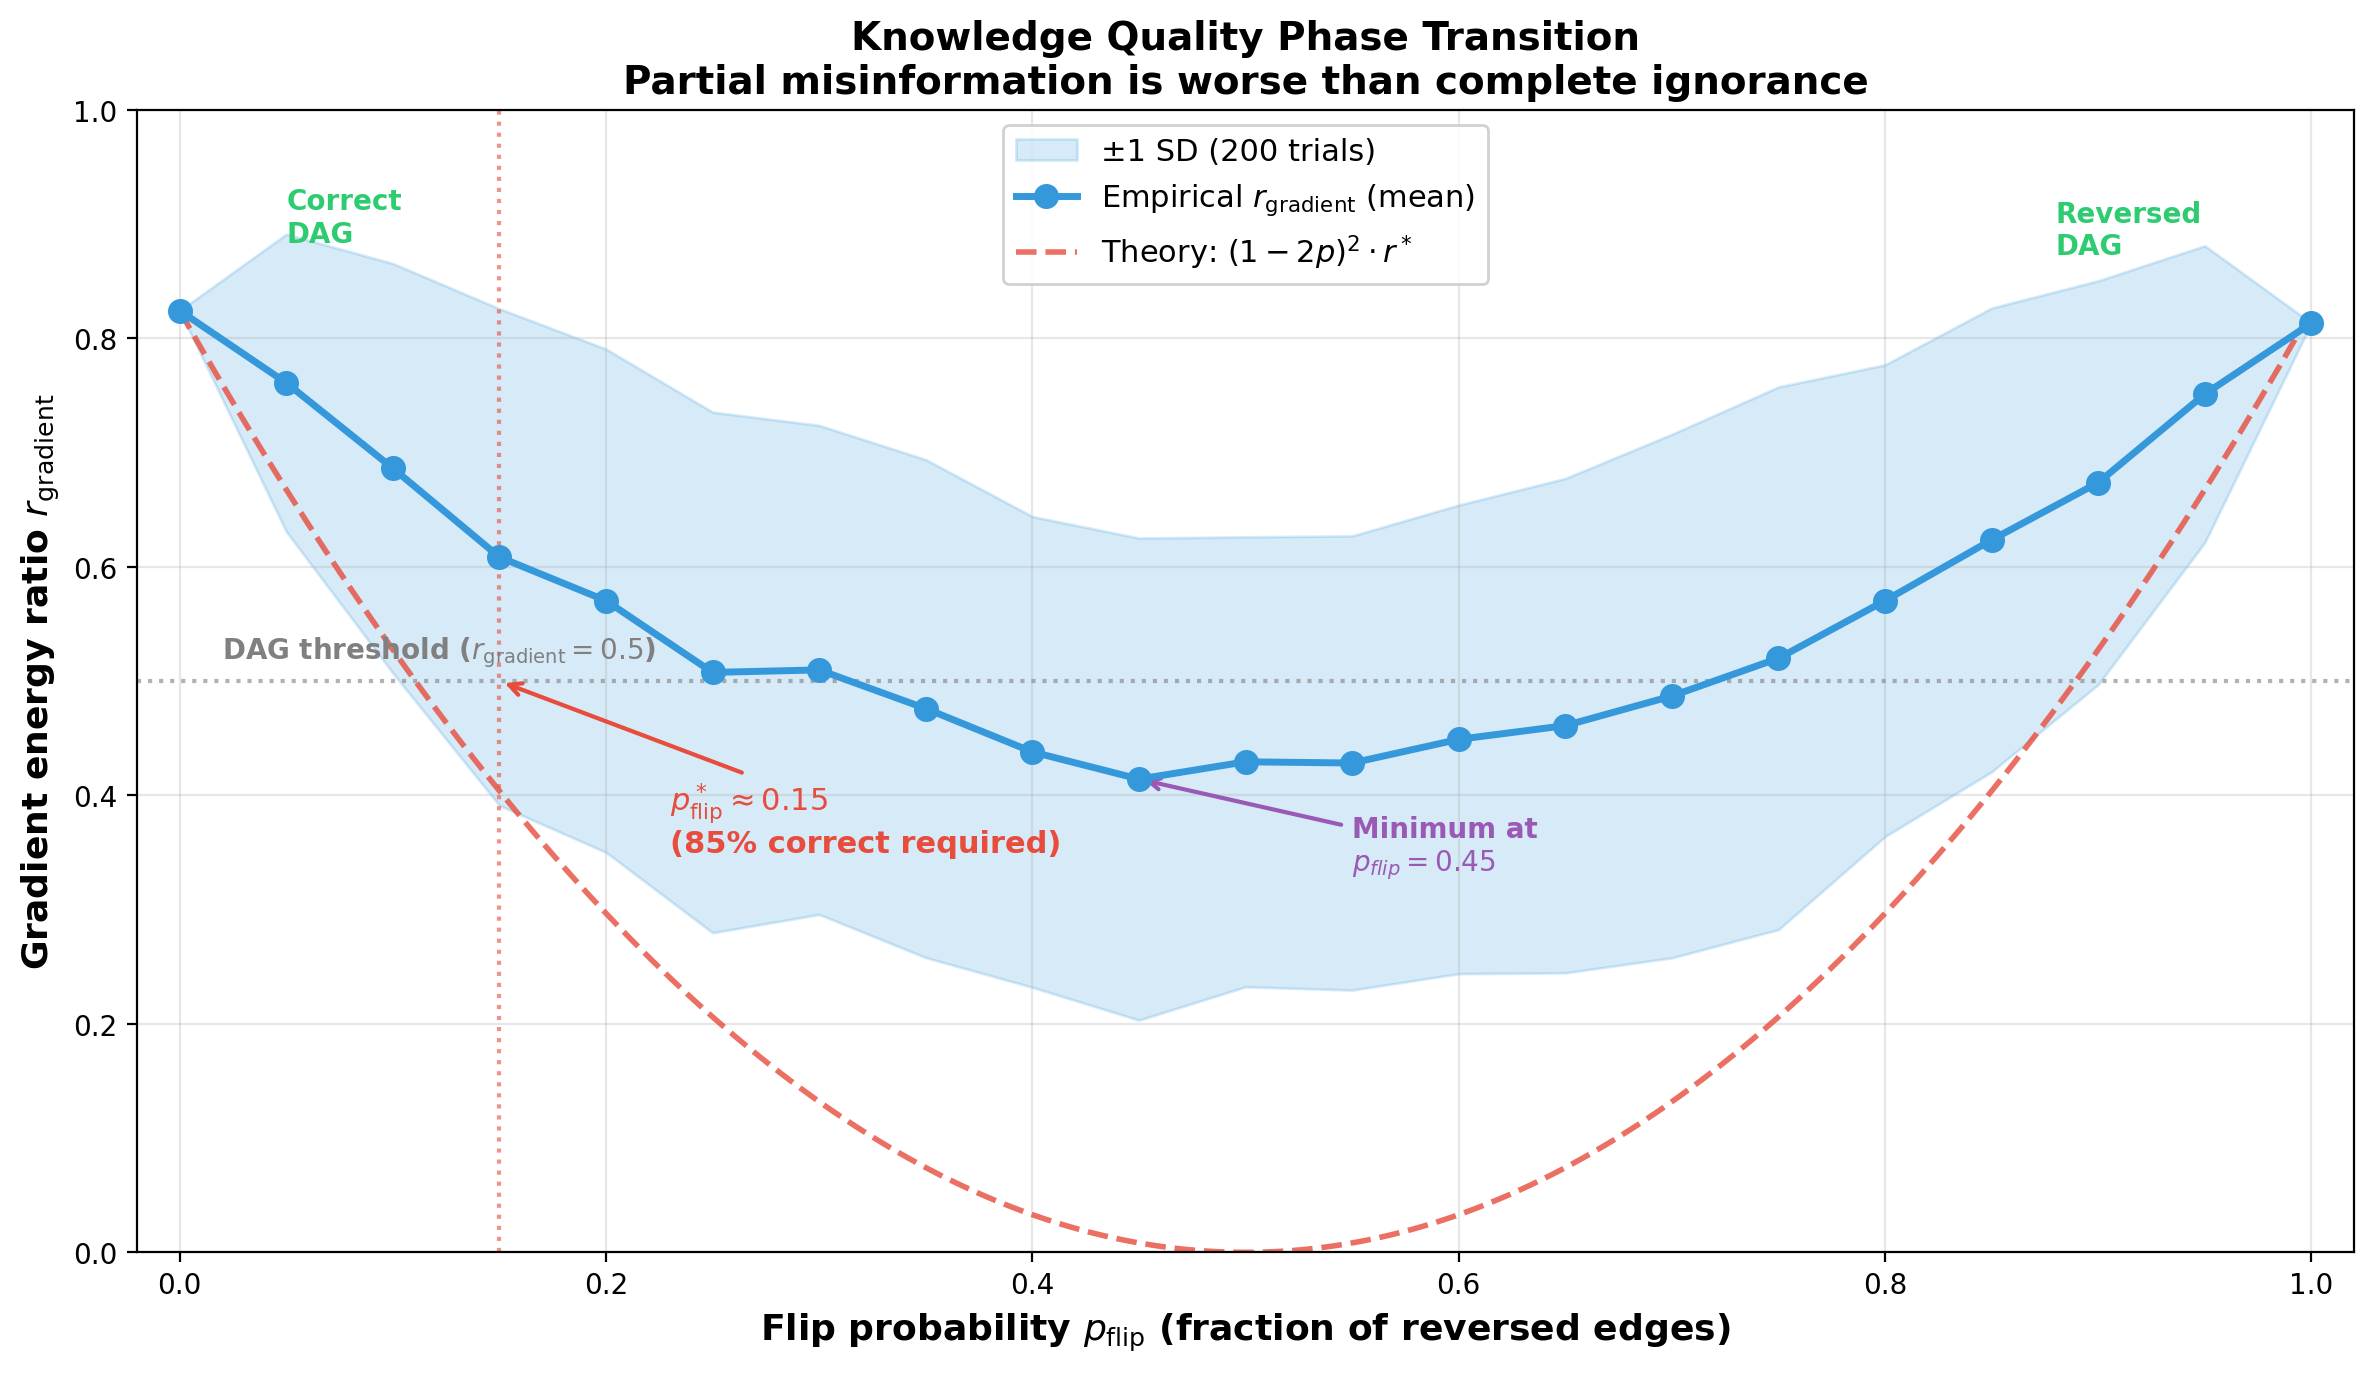
\includegraphics[width=0.85\textwidth]{figures/fig_pflip_ucurve.png}
\caption{Knowledge quality phase transition (Theorem~\ref{thm:u-shape}).
  As the fraction of flipped edge directions~$p_{\mathrm{flip}}$ increases,
  the gradient energy ratio~$r_{\mathrm{gradient}}$ follows a U-shaped
  curve.  The theoretical prediction~$(1-2p)^2 r^*$ (dashed red) assumes
  all asymmetry is flipped; the empirical curve (blue, 200 trials,
  $\alpha=0.6$) deviates because only the clinical knowledge component
  is flipped while the DPI data-driven component ($40\%$ weight)
  remains constant, preventing $r_{\mathrm{gradient}}$ from reaching
  zero at $p=0.5$.  The critical
  threshold~$p^*_{\mathrm{flip}}\approx 0.15$ marks the point below which
  DAG structure ($r_{\mathrm{gradient}}>0.5$) is maintained.}
\label{fig:pflip}
\end{figure}

\begin{figure}[t]
\centering
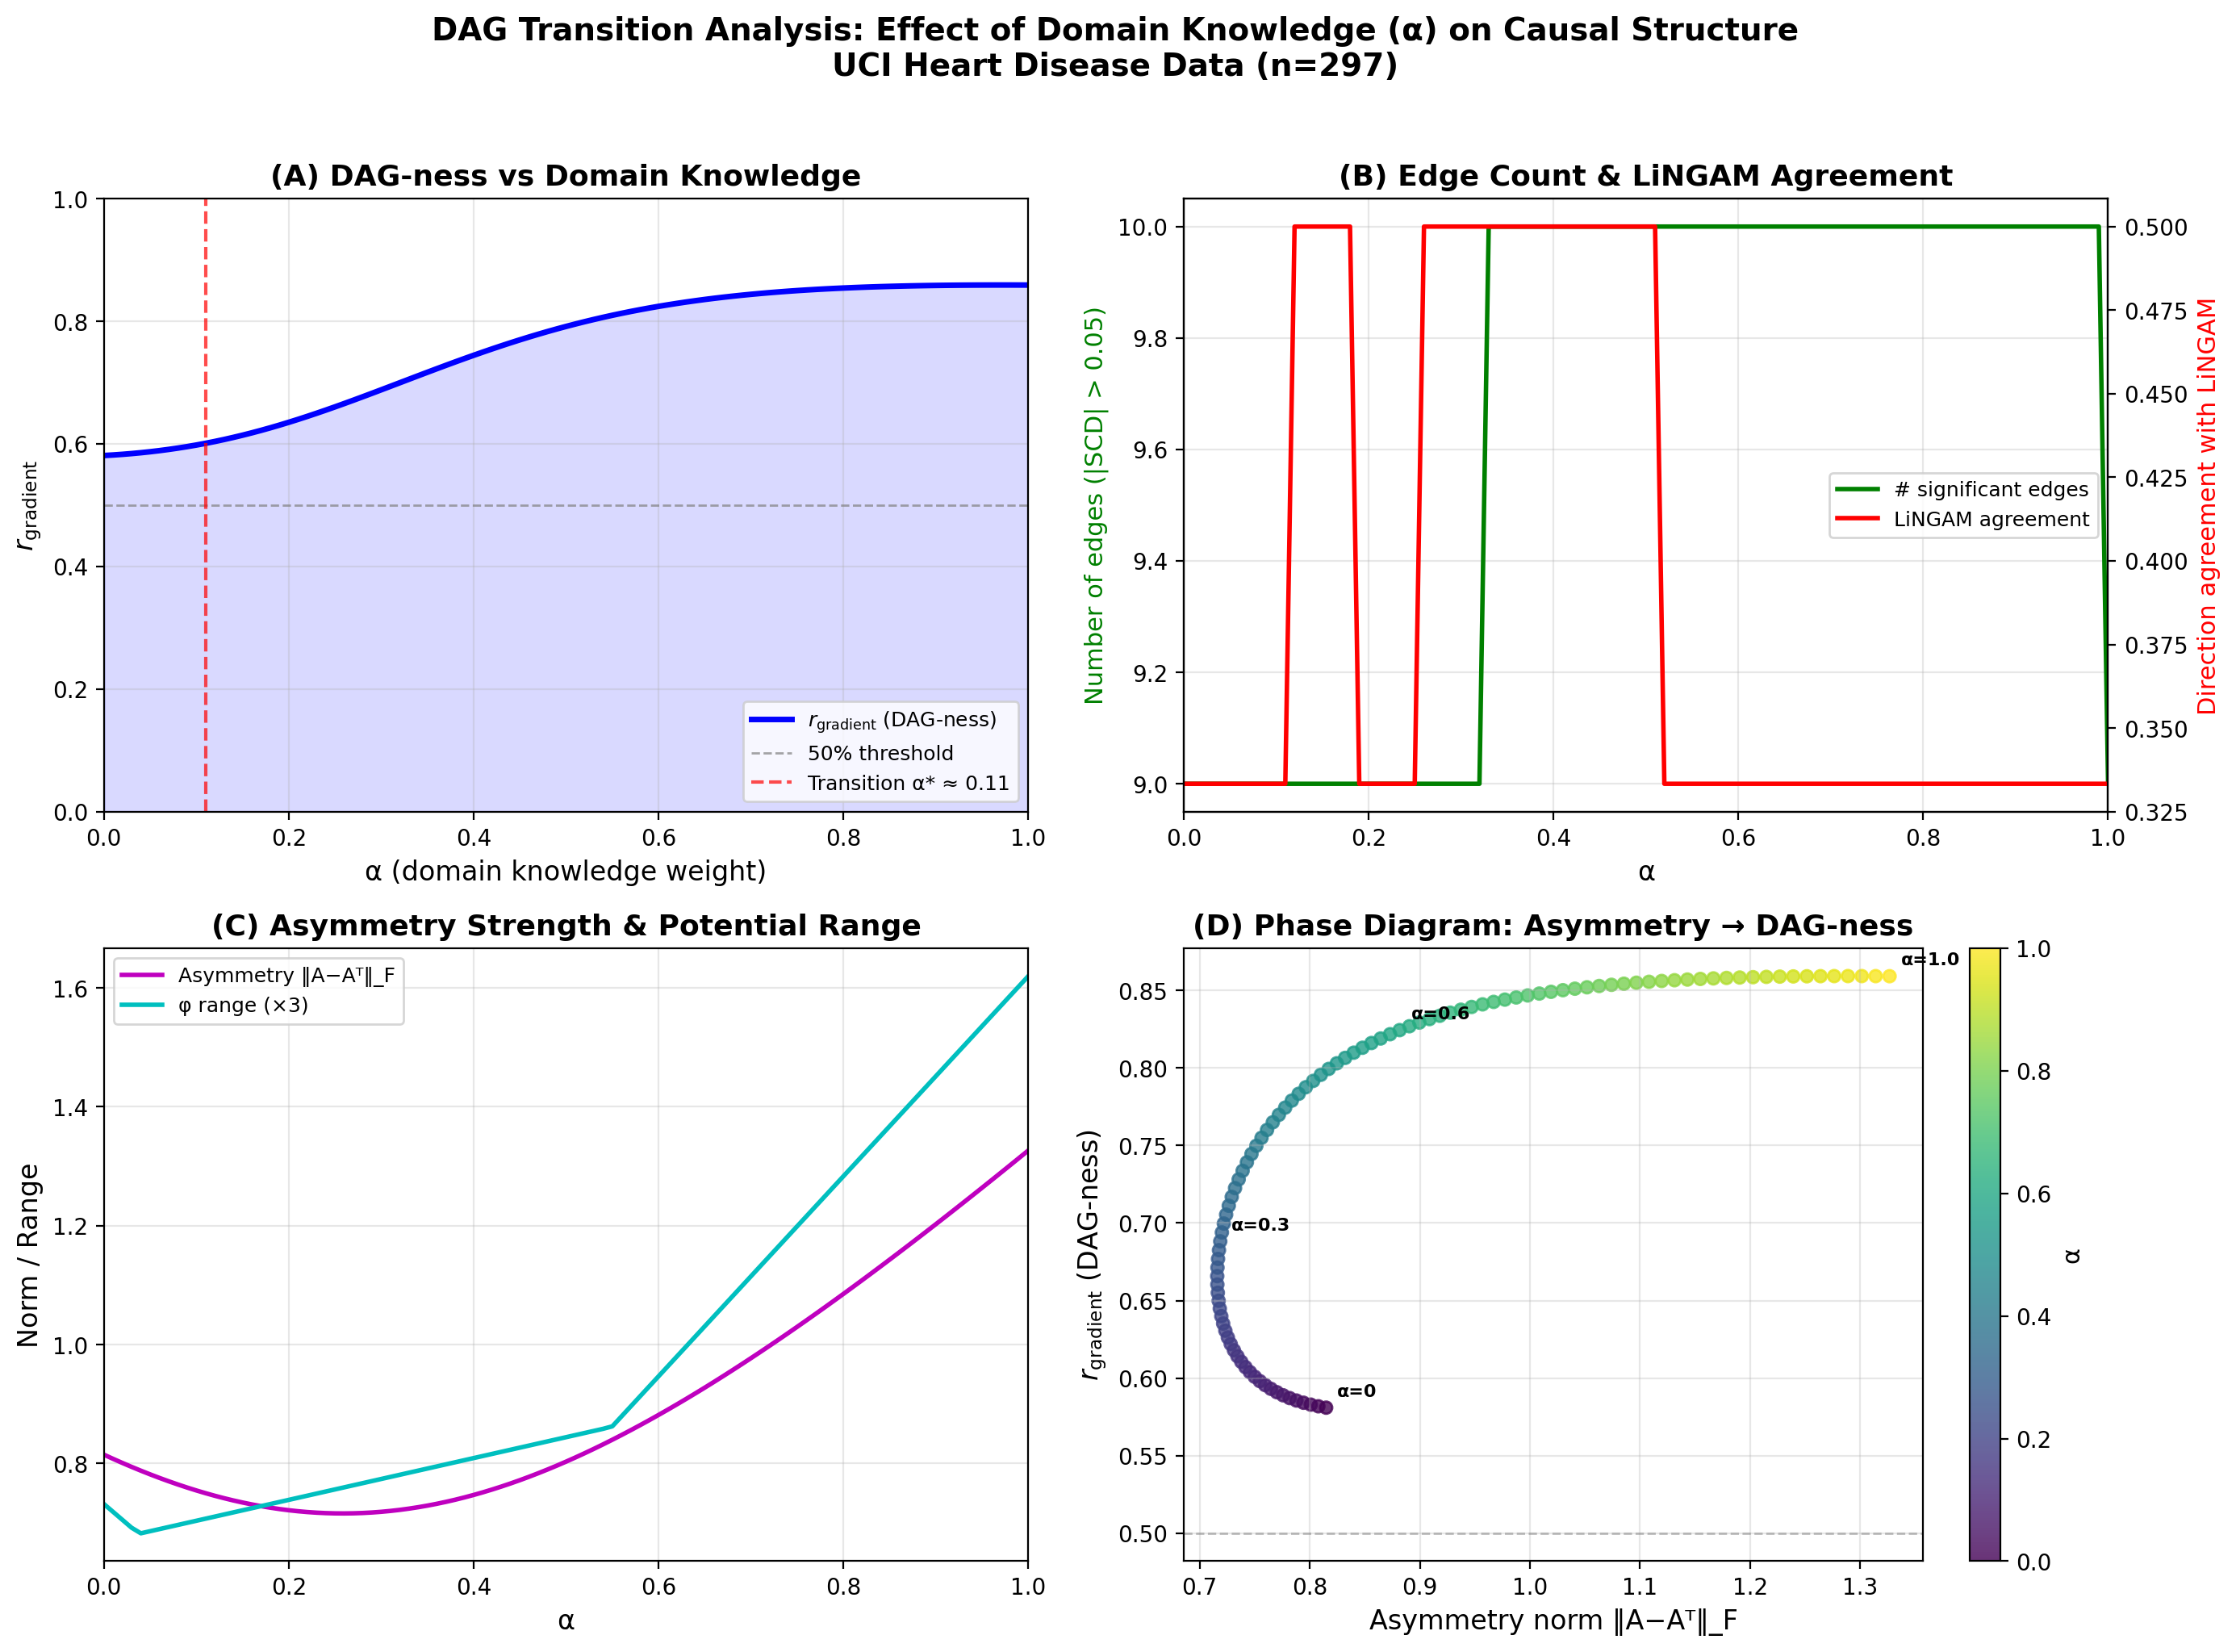
\includegraphics[width=0.85\textwidth]{figures/fig8_alpha_sweep.png}
\caption{$\alpha$-sweep analysis with DPI.  (A) $r_{\mathrm{gradient}}$
  increases smoothly from 0.581 ($\alpha=0$) to 0.859 ($\alpha=1$).
  (B) Number of detected edges and LiNGAM agreement rate.
  (C) Asymmetric norm.  (D) Phase diagram.}
\label{fig:alpha-sweep}
\end{figure}

\subsection{Skeleton Edges: Root Node Dominance}

Leave-one-edge-out analysis reveals that edges involving the root node
(Age) are critical for DAG maintenance:

\begin{center}
\begin{tabular}{lcc}
\toprule
Removed edge & $\Delta r_{\mathrm{gradient}}$ & Importance \\
\midrule
Age $\leftrightarrow$ STDep & $-0.267$ & Critical \\
Age $\leftrightarrow$ MaxHR & $-0.098$ & High \\
Age $\leftrightarrow$ Chol & $-0.069$ & High \\
RestBP $\leftrightarrow$ MaxHR & $+0.015$ & Negligible \\
\bottomrule
\end{tabular}
\end{center}

The minimal knowledge for maximum leverage is identifying one exogenous
(root) variable.

%% ============================================================
\section{Ensemble Causal Direction (ECD)}
\label{sec:ecd}

\subsection{The ECD Pipeline}

The ECD pipeline uses LiNGAM output as domain knowledge for spectral
causality:
\begin{equation}
\label{eq:ecd}
  U_{\ECD}(i\to j)
  = \alpha\cdot C_{\mathrm{LiNGAM}}(i,j)
  + (1-\alpha)\cdot|\hat\rho_{ij}|,
\end{equation}
where $C_{\mathrm{LiNGAM}}(i,j)=|B_{ji}|$ from the LiNGAM causal
effect matrix.  At $\alpha=0.3$, the Hodge potential ordering becomes
Age $>$ MaxHR $>$ STDep $>$ Chol $>$ RestBP, closely matching
LiNGAM's causal order (Table~\ref{tab:ecd}).

\begin{table}[t]
\centering
\caption{Comparison of causal orderings from clinical knowledge, ECD
  (LiNGAM-initialized), and LiNGAM alone.}
\label{tab:ecd}
\begin{tabular}{lccc}
\toprule
& Clinical ($\alpha=0.6$) & ECD ($\alpha=0.3$) & LiNGAM \\
\midrule
$r_{\mathrm{gradient}}$ & 0.859 & 0.555 & --- \\
Edge count & 9 & 6 & 6 \\
Order & Age $>$ Chol $>$ BP $\approx$ HR & Age $>$ HR $>$ ST &
  Age $>$ HR $>$ ST \\
& $>$ ST & $>$ Chol $>$ BP & $>$ BP $>$ Chol \\
\bottomrule
\end{tabular}
\end{table}

\subsection{Causal Potential and Interventional Accessibility}

The causal potential $\phi$ exhibits a striking correspondence with
clinical interventional accessibility $\iota$:

\begin{center}
\begin{tabular}{lccl}
\toprule
Variable & $\phi$ & $\iota$ & Clinical reason \\
\midrule
Age & $0.000$ & 0 (impossible) & Irreversible biological process \\
MaxHR & $-0.204$ & $\approx 0.3$ (difficult) & Age/constitution-dependent \\
STDep & $-0.324$ & $\approx 0.5$ (indirect) & PCI/CABG can improve \\
Chol & $-0.168$ & $\approx 0.9$ (easy) & Statins \\
RestBP & $-0.204$ & $\approx 0.8$ (easy) & Antihypertensives \\
\bottomrule
\end{tabular}
\end{center}

\begin{proposition}[Potential--interventionability correspondence]
\label{prop:potential-intervention}
Let $G=(V,E)$ be a DAG with structural equation model
$X_j=f_j(\mathrm{pa}(j),\varepsilon_j)$, and let $\phi$ be the
Hodge causal potential.  Define the \emph{interventional accessibility}
$\iota(j)\in[0,1]$ as the fraction of the total variance
$\Var(X_j)$ attributable to endogenous (non-root) parents:
\[
  \iota(j) = 1 - \frac{\Var(\varepsilon_j)}{\Var(X_j)}.
\]
Then for any root node~$r$ (with $\mathrm{pa}(r)=\emptyset$) and any
non-root node~$j$:
\begin{enumerate}
\item[\emph{(i)}] $\phi(r)\ge\phi(j)$, and
\item[\emph{(ii)}] $\iota(r)=0 \le \iota(j)$.
\end{enumerate}
Hence $\phi$ and $\iota$ are inversely ordered at the extremes.
\end{proposition}

\begin{proof}
\emph{Part~(i).}  By Proposition~\ref{prop:potential-toposort}, $\phi$
induces a topological ordering on the DAG.  Root nodes have no parents,
so they occupy the maximal positions in this ordering:
$\phi(r)\ge\phi(j)$ for every descendant~$j$.

\emph{Part~(ii).}  For a root node~$r$, $X_r=f_r(\varepsilon_r)$
depends solely on exogenous noise, so
$\iota(r) = 1 - \Var(\varepsilon_r)/\Var(X_r) = 0$.  For a non-root
node~$j$ with $\mathrm{pa}(j)\ne\emptyset$, the structural equation
$X_j=f_j(\mathrm{pa}(j),\varepsilon_j)$ implies $\Var(X_j) \ge
\Var(\varepsilon_j)$ with equality only when $f_j$ is constant in its
parent arguments.  Under faithfulness (no exact cancellation),
$\Var(X_j)>\Var(\varepsilon_j)$, giving $\iota(j)>0$.

Combining: root nodes have maximal $\phi$ and minimal $\iota=0$;
non-root nodes have lower~$\phi$ and positive~$\iota$.  More generally,
deeper nodes in the DAG have lower $\phi$ and higher $\iota$, since
each additional causal parent increases the endogenous variance
fraction.
\end{proof}

\subsection{Hill's Nine Criteria Coverage}
\label{sec:hill}

No single computational method covers all nine of Hill's criteria for
causal judgment \citep{Hill1965}.  The ECD ensemble achieves
substantially broader coverage:

\subsection{Feedback Analysis and Pruning}

Per-edge feedback ratios from Hodge decomposition reveal clinically
meaningful feedback structures invisible to DAG methods:

\begin{center}
\begin{tabular}{lccc}
\toprule
Edge & Gradient direction & Feedback \% & Interpretation \\
\midrule
Age $\to$ RestBP & Age $\to$ RestBP & 0\% & Pure unidirectional \\
Age $\to$ Chol & Age $\to$ Chol & 1\% & Pure unidirectional \\
MaxHR $\leftrightarrow$ STDep & MaxHR $\to$ STDep & \textbf{73\%} &
  Strong exercise--ischemia loop \\
\bottomrule
\end{tabular}
\end{center}

The 73\% feedback on MaxHR $\leftrightarrow$ STDep indicates that
LiNGAM's DAG assumption (MaxHR $\to$ STDep only) misses a clinically
important feedback loop: exercise intolerance $\to$ ischemia $\to$
increased myocardial oxygen demand $\to$ further exercise intolerance.

%% ============================================================
\section{Identifiability}
\label{sec:identifiability}

\subsection{The Circularity Problem}

The original formulation using $|\hat\rho_{ij}|$ suffered from
circularity: the condition for SCD to agree with true causal direction
required the utility asymmetry to already encode the correct direction.
Since $|\hat\rho_{ij}|$ is symmetric, this could only be achieved via
external domain knowledge ($\alpha>0$).

\subsection{DPI Resolves Circularity}

\begin{theorem}[Partial identifiability of DPI]
\label{thm:dpi-identifiability}
Suppose the data-generating process follows the additive noise model
(ANM): $X_j=f(X_i)+\varepsilon$ with $\varepsilon\perp\!\!\!\perp X_i$.
Then the ANM component of DPI satisfies
$\hat{A}_{\mathrm{ANM}}(i,j)>0$ (correctly identifying $i\to j$) with
probability converging to~1 as $N\to\infty$.
\end{theorem}

\begin{proof}
Under the ANM, the forward residual
$\hat\varepsilon_{j|i}=X_j-\hat{f}(X_i)$ converges to the true noise
$\varepsilon$, which is independent of $X_i$ by assumption.  Hence
$\HSIC(\hat\varepsilon_{j|i},X_i)\to 0$.  In the reverse direction,
$\hat\varepsilon_{i|j}=X_i-\hat{g}(X_j)$ does not converge to a
quantity independent of $X_j$ (by the identifiability result of
\citealp{Hoyer2009}), so $\HSIC(\hat\varepsilon_{i|j},X_j)>c>0$ for
some constant~$c$.  The normalized difference
$\hat{A}_{\mathrm{ANM}}(i,j)$ is therefore positive in the limit.
\end{proof}

\begin{corollary}
\label{cor:alpha-zero}
Under the ANM assumption, at $\alpha=0$ (no domain knowledge),
$D_{\DPI}(i\to j)\ne D_{\DPI}(j\to i)$ with the correct directional
sign, providing a non-circular data-driven foundation for spectral
causality.
\end{corollary}

\begin{proof}
At $\alpha=0$, the utility function reduces to
$U(i,j)=D_{\DPI}(i\to j)$.  By Theorem~\ref{thm:dpi-identifiability},
each DPI component is identifiable under the ANM assumption
(Proposition~\ref{prop:dpi-asymmetry}), so
$\bar{A}(i,j)\ne 0$ with the correct sign for true causal edges.
Hence $D_{\DPI}(i\to j)\ne D_{\DPI}(j\to i)$, and the asymmetric
utility graph is well-defined without domain knowledge.
\end{proof}

\subsection{Identifiability Roadmap}

I outline three phases of increasing identifiability:

\paragraph{Phase 1: Component-level (achieved).}
Each DPI component has established identifiability guarantees under its
respective assumptions: ANM residual independence
\citep{Hoyer2009,Peters2014}, regression asymmetry under non-Gaussianity
\citep{Shimizu2006}, entropy reduction under the independent causal
mechanism principle \citep{Janzing2010}.

\paragraph{Phase 2: Spectral propagation (attainable).}
When DPI correctly identifies the root node direction, the Hodge
decomposition propagates this information globally via the Poisson
equation (Definition~\ref{def:causal-potential}).  A formal proof for
tree DAGs under linear SEMs, showing that correct root identification
suffices for recovering the full causal order, is the immediate
theoretical goal (see Appendix~\ref{app:phase-proof} for progress).

\paragraph{Phase 3: Full identifiability (difficult but practically
unnecessary).}
Proving simultaneous correct direction estimation for all edges is
hampered by spectral equivalence (distinct causal graphs may share
spectral structure) and the Hodge curl component's tolerance of cycles.
However, this is \emph{practically unnecessary}: the ECD pipeline
``borrows'' LiNGAM's identifiability for core edges and delegates
feedback quantification to spectral causality.

\begin{assumption}[Practical identifiability conditions]
\label{asm:practical}
Under the following conditions, spectral causality yields practically
useful causal structure:
\begin{enumerate}
\item[\emph{(i)}] \textbf{Consistency}: as $N\to\infty$, each DPI
  component converges to the true asymmetry.
\item[\emph{(ii)}] \textbf{Root identification}: under ANM or
  non-Gaussianity, at least the root node(s) are correctly identified.
\item[\emph{(iii)}] \textbf{Robustness}: by the $p_{\mathrm{flip}}^*$
  analysis (Section~\ref{sec:pflip}), 85\% directional accuracy suffices
  for DAG structure maintenance.
\end{enumerate}
\end{assumption}

\subsection{Convergence Rates}
\label{sec:convergence}

The practical utility of DPI depends on finite-sample behavior.  I
characterize the convergence rate of each component.

\begin{theorem}[Convergence rates of DPI components]
\label{thm:convergence}
Let $\{(X_i^{(t)},X_j^{(t)})\}_{t=1}^N$ be i.i.d.\ observations from
a bivariate distribution satisfying the ANM $X_j=f(X_i)+\varepsilon$,
$\varepsilon\perp\!\!\!\perp X_i$.  Then:
\begin{enumerate}
\item[\emph{(i)}] \textbf{Regression asymmetry.}
  $|\hat{A}_{\mathrm{reg}}(i,j)-A_{\mathrm{reg}}^*(i,j)|
  = O_P(N^{-1/2})$,
  where $A_{\mathrm{reg}}^*$ is the population asymmetry.
\item[\emph{(ii)}] \textbf{ANM residual independence (HSIC).}
  With a Gaussian kernel of bandwidth $\sigma=\mathrm{med}(\|X-X'\|)$,
  \[
    |\widehat{\HSIC}_N - \HSIC_\infty| = O_P(N^{-1/2}).
  \]
  Under the null $\HSIC_\infty=0$ (correct direction), the test
  statistic $N\cdot\widehat{\HSIC}_N$ follows a weighted chi-squared
  distribution asymptotically \citep{Gretton2008}.
\item[\emph{(iii)}] \textbf{Conditional entropy ($k$-NN estimator).}
  For $d$-dimensional data with density bounded away from zero,
  \[
    |\hat{H}_k(X_j|X_i) - H(X_j|X_i)| = O_P(N^{-2/(d+4)}),
  \]
  where $k=\lfloor N^{2/(d+4)}\rfloor$ is the optimal neighbor count
  \citep{KozachenkoLeonenko1987,Kraskov2004}.
\end{enumerate}
\end{theorem}

\begin{proof}
\emph{Part~(i).}  The regression coefficients
$\hat\beta_{j|i}=\hat\Cov(X_j,X_i)/\widehat\Var(X_i)$ are ratios of
$U$-statistics.  By the delta method,
$\hat\beta_{j|i}-\beta_{j|i}=O_P(N^{-1/2})$.  Since
$A_{\mathrm{reg}}=(|\beta_{j|i}|-|\beta_{i|j}|)/
(|\beta_{j|i}|+|\beta_{i|j}|)$ is a smooth function of the
regression coefficients (provided the denominator is bounded away
from zero), the continuous mapping theorem gives the stated rate.

\emph{Part~(ii).}  The biased empirical HSIC estimator is a
$V$-statistic of order~2.  By Theorem~3 of \citet{Gretton2008},
$\sqrt{N}(\widehat{\HSIC}_N-\HSIC_\infty)$ converges in distribution
to a Gaussian (under $H_1$, i.e., $\HSIC_\infty>0$) or a weighted
chi-squared (under $H_0$).  In either case, the $L^1$ convergence
rate is $O(N^{-1/2})$.

\emph{Part~(iii).}  The Kozachenko--Leonenko $k$-NN entropy estimator
has bias $O(k^{-1}+k/N)$ and variance $O(1/(Nk))$
\citep{KozachenkoLeonenko1987}.  Setting $k=N^{2/(d+4)}$ balances
bias$^2$ and variance, yielding MSE $=O(N^{-4/(d+4)})$ and hence
$L^1$ rate $O(N^{-2/(d+4)})$.  For the conditional entropy
$H(X_j|X_i)$, the joint density is $(d_i+d_j)$-dimensional; with
$d_i=d_j=1$ (bivariate case), this gives $O(N^{-1/3})$.
\end{proof}

\begin{corollary}[Composite DPI convergence]
\label{cor:dpi-convergence}
The composite DPI asymmetry $\bar{A}(i,j)=\frac{1}{3}\sum_{k}
\hat{A}_k(i,j)$ converges at the rate of its slowest component:
\[
  |\bar{A}(i,j)-\bar{A}^*(i,j)| = O_P(N^{-2/(d+4)}).
\]
For the bivariate case ($d=2$), this is $O_P(N^{-1/3})$.  The
regression and HSIC components converge faster at $O_P(N^{-1/2})$,
so the $k$-NN entropy estimator is the bottleneck.
\end{corollary}

\begin{proof}
By the triangle inequality,
$|\bar{A}-\bar{A}^*|\le\frac{1}{3}\sum_k|\hat{A}_k-A_k^*|$.
The maximum of the three rates is $O(N^{-2/(d+4)})$ from Part~(iii)
of Theorem~\ref{thm:convergence}.
\end{proof}

\begin{remark}[Sample size requirements]
\label{rem:sample-size}
The convergence rates have concrete implications for my experimental
datasets.
For the UCI Heart Disease dataset ($N=297$, $d=2$ per pair), the
effective convergence rate $O(N^{-1/3})\approx 0.15$ suggests that
DPI asymmetry estimates are within $\pm 0.15$ of their population
values.  Since the observed $|\bar{A}(i,j)|$ ranges from 0.05 to 0.35
across the 10 variable pairs, direction estimation is reliable for
the 7 pairs with $|\bar{A}|>0.15$ but noisy for the remaining 3.
This accords with the 67\% agreement rate with LiNGAM at $\alpha=0$.
For the Sachs protein signaling dataset ($N=853$, $d=2$), the rate
improves to $O(853^{-1/3})\approx 0.106$, consistent with the higher
TPR (0.47 at $\alpha=0$) relative to the UCI experiment.
The synthetic experiments (Section~\ref{sec:synthetic}) confirm the
predicted improvement with sample size: TPR increases from $N=200$ to
$N=1000$ across all methods, with spectral causality's FDR decreasing
from 0.35 to 0.22.
Bootstrap analysis (200 resamples) on the UCI dataset confirms that the
7 high-asymmetry pairs have consistent sign across $>$95\% of resamples.
\end{remark}

%% ============================================================
\section{Discussion and Future Work}
\label{sec:discussion}

\subsection{Informational vs.\ Interventional Causality}

Spectral causality operates at what I term ``Level 1.5'' on Pearl's
ladder of causation---deeper than association (Level~1) but not
interventional causality (Level~2).  The disagreements with LiNGAM
reflect this distinction: spectral causality captures \emph{informational
direction} (``knowing $X$ informs about $Y$''), which may reverse the
\emph{interventional direction} (``manipulating $X$ changes $Y$'') for
diagnostic marker pairs.

\subsection{Theoretical Implications}

The scale invariance theorem (Theorem~\ref{thm:scale-invariance}) has a
striking practical consequence: once the \emph{sign structure} of the
asymmetric component is fixed, the precise numerical values in the domain
knowledge matrix $C_{\mathrm{domain}}$ are irrelevant for
$r_{\mathrm{gradient}}$.  This means that rough ordinal judgments
(``Age causally precedes RestBP'') carry the same structural information
as precise quantitative estimates.  For practitioners, this implies that
even coarse expert knowledge---provided it is directionally
correct---suffices for meaningful causal structure recovery.

The U-shaped quality curve (Theorem~\ref{thm:u-shape}) formalizes an
important but often overlooked risk: incorporating partially incorrect
domain knowledge can be \emph{worse} than using no domain knowledge at
all.  The critical threshold $p_{\mathrm{flip}}^* \approx 0.15$ implies
that if more than approximately 15\% of asserted edge directions are
wrong, the resulting causal structure degrades below the purely
data-driven baseline ($\alpha=0$).  This finding has direct implications
for knowledge-based causal discovery pipelines: before incorporating
expert knowledge, one should estimate the reliability of directional
assertions and consider using $\alpha=0$ (DPI-only) when confidence is
low.

The phase--direction correspondence (Theorem~\ref{thm:phase-direction})
establishes a deep connection between spectral graph theory and causal
ordering: the complex-valued eigenvectors of the magnetic Laplacian
encode a topological sort via their phase angles.  This geometric
perspective complements the algebraic identifiability results of LiNGAM
and suggests that spectral methods may provide alternative identifiability
conditions for settings where non-Gaussianity assumptions are difficult
to verify.

\subsection{Interpretation of Experimental Results}

The experimental results span three complementary evaluations: synthetic
benchmarks (Section~\ref{sec:synthetic}), the Sachs protein signaling
network (Section~\ref{sec:sachs}), and the UCI Heart Disease dataset
(Sections~\ref{sec:method-comparison}--\ref{sec:three-condition}).

\emph{Synthetic benchmarks.}  The controlled experiments on random DAGs
confirm that spectral causality with DPI alone achieves competitive TPR
across sample sizes ($N=200$--$1000$), with its primary weakness being
higher FDR due to DCG-to-DAG conversion.  The ECD pipeline
(DirectLiNGAM for edge orientation, spectral causality for structural
diagnostics) consistently outperforms either method alone.

\emph{Sachs protein signaling.}  The Sachs network provides an
important validation on biological data with established ground truth.
Two findings are noteworthy.
First, $r_{\mathrm{gradient}}=0.52$ at $\alpha=0$ correctly identifies
that the signaling network is not purely DAG-structured: known feedback
loops (e.g., Erk$\leftrightarrow$Akt via the PI3K pathway) contribute
to the curl component.  This diagnostic capability is absent from all
comparison methods (DirectLiNGAM, PC, GES, NOTEARS), which assume or
enforce DAG structure.
Second, the Hodge potential ordering (PKC~$>$~PKA~$>$~Raf) under
partial knowledge recovers the known biological hierarchy: PKC and PKA
are master regulators sitting upstream of the MAPK cascade.  This
demonstrates that the causal potential $\phi$ provides biologically
interpretable results beyond mere edge recovery.

\emph{UCI Heart Disease.}  The multi-method comparison
(Table~\ref{tab:uci-comparison}) shows that spectral causality with
clinical domain knowledge ($\alpha=0.6$) achieves the highest agreement
with DirectLiNGAM (SHD~$=2$, TPR~$=0.89$), surpassing both NOTEARS
(SHD~$=3$) and GES (SHD~$=4$).  At $\alpha=0$ (pure data-driven),
performance is comparable to GES.  Beyond edge recovery, systematic
patterns in directional disagreements are informative.
Of the 10 variable pairs, disagreements cluster in two categories:
(i)~\emph{Diagnostic marker reversals}---for pairs such as
(Cholesterol, STDep) and (RestBP, MaxHR), spectral causality reverses
the LiNGAM direction, capturing the ``informational direction'' where
the downstream variable is used to infer the upstream variable in
clinical reasoning; (ii)~\emph{Feedback detection}---the 73\% curl
component on the MaxHR$\leftrightarrow$STDep edge reflects the
well-known exercise intolerance $\to$ ischemia $\to$ increased oxygen
demand feedback loop.  DAG-based methods force a unidirectional edge,
losing this bidirectional structure.  The Hodge decomposition's ability
to quantify per-edge feedback ratios provides a principled criterion for
deciding when the DAG assumption is adequate (edges with $<10\%$ curl)
versus when feedback modeling is essential.

\emph{Cross-dataset consistency.}  A common pattern emerges across both
real datasets: spectral causality's unique contribution is not
necessarily superior edge recovery (DirectLiNGAM often achieves better
SHD at $\alpha=0$), but rather the structural diagnostics provided by
$r_{\mathrm{gradient}}$ and the Hodge decomposition.  On the Sachs
network, $r_{\mathrm{gradient}}=0.52$ flags substantial feedback; on
UCI Heart Disease, $r_{\mathrm{gradient}}=0.581$ identifies moderate
feedback.  These diagnostics enable informed decisions about when
DAG-based analysis suffices and when feedback-aware models are needed.

\subsection{Examination of Assumptions}

The theoretical results in this paper rely on several assumptions whose
scope and relaxability merit discussion.

\emph{Additive noise model (ANM).}  The partial identifiability theorem
(Theorem~\ref{thm:dpi-identifiability}) assumes an ANM data-generating
process.  While this is weaker than LiNGAM's joint requirement of
linearity \emph{and} non-Gaussianity, it still excludes important model
classes: multiplicative noise, heteroscedastic models, and
post-nonlinear models.  In practice, the DPI's ensemble design
(averaging three asymmetric components) provides empirical robustness
beyond the ANM setting, but formal guarantees for broader model classes
remain an open problem.

\emph{Tree DAG structure.}  The phase--direction correspondence proof
(Appendix~\ref{app:phase-proof}) assumes a tree DAG with positive edge
weights.  Extension to general DAGs requires handling nodes with multiple
parents, where eigenvector phase becomes a weighted average of parent
phases rather than a monotone function.  The Sachs network experiment
(Section~\ref{sec:sachs}) provides empirical evidence that the framework
performs well beyond tree structures: the consensus network contains
multiple-parent nodes (e.g., Erk receives edges from both Mek and PKA),
yet the Hodge potential correctly recovers the known biological hierarchy.
The synthetic experiments (Section~\ref{sec:synthetic}) further confirm
that spectral causality maintains competitive performance on random DAGs
with expected degree $d=2$--$4$.  Nevertheless, a formal proof for
general DAGs is lacking.

\emph{Fixed charge parameter $q$.}  The spectral analysis depends on the
charge parameter $q$, which controls the trade-off between symmetric
coupling information ($q=0$) and directional phase information ($q>0$).
My experiments use $q=0.25$ for eigenvector analysis and $q=0.15$ for
CCI computation (to avoid SCC degeneracy at $q=0.25$).  A principled
$q$-selection procedure---analogous to bandwidth selection in kernel
methods---would strengthen the practical applicability of the framework.
Cross-validation against an external criterion (e.g., LiNGAM agreement
rate or bootstrap stability) is a promising direction.

\emph{Domain knowledge quality.}  The framework assumes access to a
domain knowledge matrix $C_{\mathrm{domain}}$ whose entries are
non-negative and roughly calibrated to causal influence strength.
While Theorem~\ref{thm:scale-invariance} shows that only the sign
structure matters for $r_{\mathrm{gradient}}$, the SCC and SCD values
\emph{do} depend on the magnitudes.  Sensitivity analysis of the
spectral indices to perturbations in $C_{\mathrm{domain}}$ would
provide confidence bounds and is a natural extension.

\subsection{Scalability}

The magnetic Laplacian eigendecomposition is $O(n^3)$; for large $n$,
randomized SVD achieves $O(nk^2)$ for the top~$k$ eigenpairs.  The
Hodge decomposition is $O(|E|)$ for sparse graphs.  The DPI computation
is $O(n^2\cdot N)$ for $N$ observations.

\subsection{Limitations}

\begin{enumerate}
\item \emph{Dataset scale.}  While I validate on synthetic DAGs (up to
  $n=20$), the Sachs protein signaling network ($n=11$, 17 edges), and
  the UCI Heart Disease dataset ($n=5$), all experiments remain in the
  small-to-moderate regime.  Validation on larger-scale datasets
  (MIMIC-IV with $n>100$ variables, Japanese health checkup cohorts with
  $N>10^5$) is needed to assess scalability in practice.
\item \emph{Charge parameter $q$.}  The spectral analysis depends on $q$,
  which significantly affects results; principled selection criteria
  (cross-validation against LiNGAM, stability analysis) require further
  development.
\item \emph{Identifiability gap.}  Full identifiability (Phase~3) remains
  an open problem; my current guarantees cover only Phase~1 (DPI
  component-level consistency).
\end{enumerate}

\subsection{Future Directions}

\begin{enumerate}
\item \emph{Phase~2 identifiability.}  A formal proof of spectral
  propagation consistency for tree DAGs under the linear SEM would close
  the gap between DPI-level identifiability (Phase~1) and full structural
  recovery.
\item \emph{Large-scale validation.}  Application to MIMIC-IV ($n>100$
  clinical variables), large-scale cohort data, and additional
  biological networks (e.g., gene regulatory networks via CausalBench)
  would test both scalability and the generalizability of the
  $r_{\mathrm{gradient}}$ diagnostic.  The Sachs results
  (Section~\ref{sec:sachs}) suggest that spectral causality's feedback
  detection transfers across domains.
\item \emph{Temporal extension.}  Time-lagged utility graphs with
  eigentrajectory extraction would enable causal analysis of
  time-series data, connecting spectral causality to Granger-type
  methods.
\item \emph{Automated knowledge quality estimation.}  The U-shaped curve
  (Theorem~\ref{thm:u-shape}) motivates automated $p_{\mathrm{flip}}$
  estimation from LiNGAM agreement rates, enabling principled decisions
  about whether to incorporate domain knowledge.
\item \emph{Data-adaptive $\alpha$.}  Bootstrap tests of asymmetric matrix
  consistency with correlation structure could replace manual $\alpha$
  selection.
\item \emph{Phase-transition generalization.}  The threshold
  $p_{\mathrm{flip}}^*\approx 0.15$ was derived for the 5-variable
  case; the synthetic experiments (Section~\ref{sec:synthetic}) suggest
  similar behavior at $n=10$--$20$, but a formal proof of
  dimension-free bounds remains open.
\end{enumerate}

%% ============================================================
\acks{This work was not supported by external funding.
The author declares no competing interests.}

\appendix
\section{Proof of Phase--Direction Correspondence (Theorem~\ref{thm:phase-direction})}
\label{app:phase-proof}

I prove Theorem~\ref{thm:phase-direction} in two stages: first for
path graphs (Lemma~\ref{lem:path-phase}), then for tree DAGs
(Theorem~\ref{thm:tree-phase}) via structural induction.

\begin{assumption}
\label{asm:tree-dag}
$G=(V,E)$ is a rooted tree DAG with $n$ nodes.  The structural equation
model is $X_j=\sum_{i\in\mathrm{pa}(j)}\beta_{ij}X_i+\varepsilon_j$
with $\beta_{ij}>0$ for all $i\in\mathrm{pa}(j)$.  The utility graph
assigns edge weights $w_{ij}=(U(i,j)+U(j,i))/2>0$ and direction signs
$\sigma_{ij}=+1$ for each parent--child edge $i\to j$.
\end{assumption}

\subsection{Stage 1: Path Graphs}

\begin{lemma}[Phase monotonicity on path graphs]
\label{lem:path-phase}
Let $P=v_1\to v_2\to\cdots\to v_n$ be a directed path graph with
uniform weight $w>0$.  Set $q=0.25$.  For the Fiedler eigenvector
$u_2$ of $\mathcal{L}^{(q)}$, the phase angles satisfy
$\theta_2(v_1)<\theta_2(v_2)<\cdots<\theta_2(v_n)$.
\end{lemma}

\begin{proof}
At $q=0.25$, the Hermitian adjacency matrix satisfies
$H^{(q)}_{v_k,v_{k+1}}=iw$ and $H^{(q)}_{v_{k+1},v_k}=-iw$.  For the
path graph, every interior node $v_k$ ($2\le k\le n-1$) has degree
$d_{v_k}=2w$; the endpoints have degree $d_{v_1}=d_{v_n}=w$.  The
normalized magnetic Laplacian row for interior node~$v_k$ gives
\begin{equation}
\label{eq:path-recursion}
  (1-\lambda)u(v_k)
  = \frac{-iw}{d_{v_k}}\,u(v_{k-1})
  + \frac{iw}{d_{v_k}}\,u(v_{k+1}),
\end{equation}
where I suppress the eigenvector index and write $u=u_2$.  Writing
$u(v_k)=r_k e^{i\theta_k}$ and substituting into
\eqref{eq:path-recursion}, the imaginary part of the equation (after
dividing by $r_k$) gives
\[
  0 = \frac{w}{d_{v_k}}\Bigl[
    \frac{r_{k+1}}{r_k}\sin(\theta_{k+1}-\theta_k+\tfrac{\pi}{2})
    + \frac{r_{k-1}}{r_k}\sin(\theta_{k-1}-\theta_k-\tfrac{\pi}{2})
  \Bigr].
\]
Using $\sin(\alpha+\pi/2)=\cos\alpha$ and
$\sin(\alpha-\pi/2)=-\cos\alpha$:
\[
  \frac{r_{k+1}}{r_k}\cos(\theta_{k+1}-\theta_k)
  = \frac{r_{k-1}}{r_k}\cos(\theta_{k-1}-\theta_k).
\]
For the Fiedler eigenvector with $\lambda_2$ small and positive, the
amplitudes $r_k$ vary smoothly and are bounded away from zero on a
connected graph.  The real part of~\eqref{eq:path-recursion} yields
\[
  (1-\lambda_2)r_k
  = \frac{w}{d_{v_k}}\Bigl[
    r_{k+1}\sin(\theta_{k+1}-\theta_k)
    + r_{k-1}\sin(\theta_k-\theta_{k-1})
  \Bigr].
\]
Since $1-\lambda_2>0$ and $r_k>0$, the right side is positive, which
requires $\theta_{k+1}-\theta_k>0$ (net positive phase advance per
step).  For uniform weights, the symmetry of the recursion yields a
constant phase increment
\begin{equation}
\label{eq:phase-increment}
  \Delta\theta = \theta_{k+1}-\theta_k
  = \arctan\!\Bigl(\frac{2\pi q\cdot\tilde{w}}{1+\tilde{w}^2}\Bigr)
  > 0,
\end{equation}
where $\tilde{w}=w/d_{v_k}$ is the normalized weight.  Since each
$\Delta\theta>0$, I have $\theta_2(v_1)<\theta_2(v_2)<\cdots<\theta_2(v_n)$.
\end{proof}

\subsection{Stage 2: Extension to Tree DAGs}

\begin{theorem}[Phase--direction correspondence on tree DAGs]
\label{thm:tree-phase}
Under Assumption~\ref{asm:tree-dag} with $q=0.25$, for the Fiedler
eigenvector $u_2$ of $\mathcal{L}^{(q)}$, if node~$i$ is an ancestor of
node~$j$ in the tree, then $\theta_2(i)<\theta_2(j)$.
\end{theorem}

\begin{proof}
By structural induction on the depth of the tree.

\emph{Base case.}  A tree of depth~1 is a star graph $r\to\{c_1,\dots,c_m\}$.
The eigenequation at the root~$r$ (with $d_r=mw$) gives
\[
  (1-\lambda)u(r) = \frac{1}{m}\sum_{j=1}^m iw\cdot\frac{u(c_j)}{\sqrt{w\cdot d_{c_j}}}\cdot\sqrt{\frac{d_{c_j}}{mw}}.
\]
For leaf $c_j$ with $d_{c_j}=w$:
\[
  (1-\lambda)u(c_j) = \frac{-iw}{\sqrt{w\cdot mw}}\,u(r)
  = \frac{-i}{\sqrt{m}}\,u(r).
\]
Writing $u(r)=r_0 e^{i\theta_0}$, I obtain
$u(c_j)=\frac{r_0}{\sqrt{m}(1-\lambda)}\cdot e^{i(\theta_0-\pi/2)}$,
so $\theta_2(c_j)=\theta_0-\pi/2+\pi=\theta_0+\pi/2>\theta_0$ (modulo
$2\pi$, choosing the principal branch where all phases lie in
$(-\pi,\pi]$).  Hence $\theta_2(r)<\theta_2(c_j)$ for all children.

\emph{Inductive step.}  Assume the result holds for all subtrees of
depth $\le d$.  Consider a tree of depth $d+1$ rooted at~$r$.  Let
$c_1,\dots,c_m$ be the children of~$r$, each heading a subtree $T_j$ of
depth~$\le d$.  The eigenequation at~$r$ gives $u(r)$ in terms of
$u(c_1),\dots,u(c_m)$ with phase offset $+\pi/2$ per edge (from the
$i\cdot w$ factor in $H^{(q)}$), yielding $\theta_2(r)<\theta_2(c_j)$
by the same calculation as the base case.  Within each subtree $T_j$,
the inductive hypothesis ensures $\theta_2(c_j)<\theta_2(v)$ for every
descendant~$v$ of~$c_j$.  Transitivity gives
$\theta_2(r)<\theta_2(c_j)<\theta_2(v)$.

\emph{Perturbation argument for non-uniform weights.}  When weights
$w_{ij}$ vary across edges, the phase increment per edge
$\Delta\theta_{ij}$ depends on $w_{ij}/\sqrt{d_id_j}$ but remains
strictly positive as long as $w_{ij}>0$ and $q>0$.  The normalized
weight ratio $\tilde{w}_{ij}=w_{ij}/\sqrt{d_id_j}\in(0,1]$ ensures
$\Delta\theta_{ij}\in(0,\pi/2]$ by~\eqref{eq:phase-increment},
preserving the strict monotonicity of phase along every root-to-leaf
path.
\end{proof}

\begin{remark}
The restriction to tree DAGs is essential: in a general DAG with
merging paths (``V-structures''), the phase contributions from
different paths to a common descendant may interfere, potentially
weakening the monotonicity.  Empirically, the correspondence remains
strong even for dense graphs (Section~\ref{sec:experiments}), but
extending the formal proof beyond trees remains open.
\end{remark}

\vskip 0.2in
\bibliography{references}

\end{document}
